% -*- coding: utf-8 -*-

\begin{chapter}{Температура, солёность и плотность}\label{chap:6}
% \chapter{Temperature, Salinity, and Density}
Потоки тепла, испарение, атмосферные осадки, речной сток, замерзание и таяние
морского льда~--- все эти явления влияют на распределение солёности 
и температуры по поверхности океана. Изменения в температуре и солёности 
могут увеличить либо уменьшить плотность воды на поверхности, что, 
в свою очередь, влияет на конвекцию. Если поверхностная вода опустится на
глубину, она сохраняет характерные соотношения между температурой и солёностью, 
что в дальнейшем помогает океанографам отслеживать глубинную циркуляцию.
Также на основе температуры, солёности и давления воды можно рассчитать её
плотность. Распределение плотности в океане прямо связано с распределением
горизонтальных градиентов давления и течений. С учетом сказанного выше,
будет важно выяснить распределение температуры, солёности и плотности в океане.
%
% Heat fluxes, evaporation, rain, river inflow, and freezing and melting
% of sea ice all influence the distribution of temperature and salinity
% at the ocean's surface. Changes in temperature and salinity can
% increase or decrease the density of water at the surface, which can
% lead to convection. If water from the surface sinks into the deeper
% ocean, it retains a distinctive relationship between temperature and
% salinity which helps oceanographers track the movement of deep
% water. In addition, temperature, salinity, and pressure are used to
% calculate density. The distribution of density inside the ocean is
% directly related to the distribution of horizontal pressure gradients
% and ocean currents.  For all these reasons, we need to know the
% distribution of temperature, salinity, and density in the ocean.

Прежде, чем начать обсуждение распределения температуры и солёности,
следует дать определение этих понятий.
%
% Before discussing the distribution of temperature and salinity, let's
% first define what we mean by the terms, especially salinity.


\begin{section}{Определение солёности}
% \section{Definition of Salinity}
В первом приближении, солёность~--- это масса вещества в граммах, 
растворенного в $1\kg$~морской воды. Из данного определения следует, 
что солёность --- величина безразмерная. Изменения содержания
растворённых солей очень малы, поэтому мы должны очень тщательно
определять солёность, используя точные и практичные методы. Чтобы
лучше понять, для чего нужна большая точность, обратимся к рис.~6.1.
Отметим, что для преобладающего количества океанской воды, диапазон значений 
солёности составляет~$34.60$--$34.80$~частей на тысячу 
(или \emph{промилле}, ‰), а разница между отдельными значениями,
соответственно, до 200 частей на миллион. 
Глубинные воды в северной части Тихого океана обладают еще меньшей 
изменчивостью, около 20 частей на миллион. Если мы хотим классифицировать 
воды с разной солёностью, нам необходимы определения и инструменты, способные 
проводить измерения с точностью до одной части на миллион. Для сравнения, 
амплитуда изменений температуры составляет около~$\degCent{1}$, 
к тому же она гораздо легче поддается измерению.
%
% At the simplest level, salinity\index{salinity|textbf} is the total
% amount of dissolved material in grams in one kilogram of sea
% water. Thus salinity is a dimensionless quantity. It has no units. The
% variability of dissolved salt is very small, and we must be very
% careful to define salinity in ways that are accurate and practical. To
% better understand the need for accuracy\index{accuracy!salinity}, look
% at figure 6.1. Notice that the range of salinity for most of the
% ocean's water is from 34.60 to 34.80 parts per thousand, which is 200
% parts per million. The variability in the deep North Pacific is even
% smaller, about 20 parts per million. If we want to classify water with
% different salinity, we need definitions and instruments accurate to
% about one part per million. Notice that the range of temperature is
% much larger, about 1\degrees{C}, and temperature is easier to measure.

Разработка практичных определений, обладающих в то же время достаточной 
точностью,  оказалась непростым делом (Lewis,1980), так что в разные моменты
времени использовались различные определения. 
%
% Writing a practical definition of salinity that has useful accuracy is
% difficult (see Lewis, 1980, for the details), and various definitions
% have been used.\\

%% Рисунок 6.1 Гистограмма температуры и солёности холодной океанской
%% воды. Высота пропорциональна объёму. Размер высочайшего пика
%% соответствует объёму в 26 кубических километров на двумерный класс
%% $\degCent{0.1}$ и $0.01\psu$. Взято из Worthington (1981).
%%
%% \begin{figure}[t!]
%% \makebox [120mm][c]{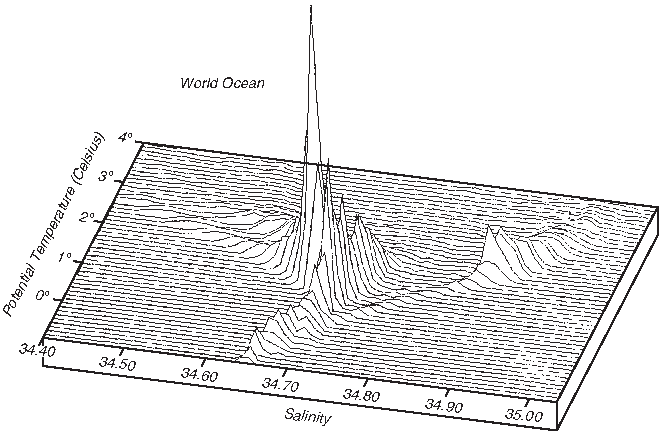
\includegraphics{salhistogram}} \footnotesize
%% Figure 6.1 Histogram of temperature \rule{0mm}{3ex}and salinity of
%% ocean water colder than 4\degrees C. Height is proportional to
%% volume. Height of highest peak corresponds to a volume of 26 million
%% cubic kilometers per bivariate class of 0.1\degrees{C} and 0.01. After
%% Worthington (1981: 47).
%% \label{fig:salhistogram}
%% \vspace{-3ex}
%% \end{figure}

\begin{paragraph}{Простое определение.} 
% \paragraph{A Simple Definition} 
Изначально солёность определяли, как <<общую массу в граммах вещества, 
растворённого в $1\kg$~морской воды>>. Это определение не слишком полезно,
так как все растворённое вещество на практике измерить почти
невозможно. Например, каким образом измерять такие летучие элементы, как газы?
%% летучие элементы???
Выпаривание морской воды также неприемлемо для получения сухого остатка, 
поскольку на его последних стадиях теряются хлориды. (Sverdrup, Johnson, and Fleming, 1942: 50).
%
% Originally salinity was defined to be the
% ``Total\index{salinity|textbf} amount of dissolved material in grams
% in one kilogram of sea water.'' This is not useful because the
% dissolved material is almost impossible to measure in practice. For
% example, how do we measure volatile material like gasses? Nor can we
% evaporate sea-water to dryness because chlorides are lost in the last
% stages of drying (Sverdrup, Johnson, and Fleming, 1942: 50).
\end{paragraph}

\begin{paragraph}{Более сложное определение.}
% \paragraph{A More Complete Definition} 
Чтобы устранить трудности, связанные с предыдущим определением, 
Международный совет по исследованию моря учредил в~1889~г.\ специальную 
комиссию, которая в 1902~г. рекомендовала понимать солёность, как 
<<количество твёрдых веществ в граммах, растворённое в $1\kg$~морской воды, 
при условии, что все галогены заменены эквивалентным количеством хлора, 
все карбонаты переведены в окислы, органическое вещество сожжено>>%
\remark{\url{http://slovari.yandex.ru/dict/bse/article/00049/64100.htm}}.
\emph{Это определение полезнее, но ним все равно сложно пользоваться 
на практике}.
%
% To avoid these difficulties, the \index{salinity!simple
% vs. complete}International Council for the Exploration of the Sea set
% up a commission in 1889 which recommended that salinity be defined as
% the ``Total amount of solid materials in grams dissolved in one
% kilogram of sea water when all the carbonate has been converted to
% oxide, the bromine and iodine replaced by chlorine and all organic
% matter completely oxidized.'' The definition was published in
% 1902. \textit{This is useful but difficult to use routinely}.
\end{paragraph}

\begin{paragraph}{Солёность, основанная на хлорности.}
% \paragraph{Salinity Based on Chlorinity} 
Так как и данное выше определение оказалось непрактичным, а солёность
прямо пропорциональна содержанию хлора в морской воде, которое, в свою 
очередь, можно точно измерить путём несложного химического анализа,
cолёность~$S$ была определена через хлорность:
\begin{equation}\label{eq:6.1}
S = 0.03 + 1.805\, \text{Cl},
\end{equation}
где \emph{хлорность}~Cl~--- 
%% <<величина, равная величине массы в единицу грамм-атомного веса 
%% серебра, которое осаждается галогенами из пробы морской воды 
%% весом~$0.3285234\kg$>> (это по Хорну) 
<<масса серебра, необходимая для полного осаждения галогенов 
в пробе воды массой~$0.3285234\kg$>>.%
\remark{Эта формула известна как <<формула Кнудсена>>.}
%
% Because the above definition was difficult \index{salinity!based on
% chlorinity}to implement in practice, because salinity is directly
% proportional to the amount of chlorine in sea water, and because
% chlorine can be measured accurately by a simple chemical analysis,
% salinity $S$ was redefined using chlorinity:
% \begin{equation}
% S = 0.03 + 1.805\, Cl
% \end{equation}
% where \textit{chlorinity}\index{chlorinity|textbf} $Cl$ is defined as
% ``the mass of silver required to precipitate completely the halogens
% in 0.328 523 4 kg of the sea-water sample.''

С ростом точности измерений погрешность формулы~(\ref{eq:6.1}) также оказалась
неприемлемой. В 1964~г. ЮНЕСКО и другие международные организации поручили
Объединенной группе по океанографическим таблицам и стандартам (ОГОТС) 
разработку более точного определения. В 1966~г. группа рекомендовала следующее 
соотношение между солёностью и хлорностью (Wooster, Lee, and Dietrich, 1969):
\begin{equation}\label{eq:6.2}
 S = 1.806\,55\,\text{Cl},
\end{equation}
которое совпадает с~(\ref{eq:6.1}) при~$S=35$.%
\remark{Также известна как <<формула ЮНЕСКО>>.}
%
% As more and more accurate measurements were made, (6.1) turned out to
% be too inaccurate. In 1964 \textsc{unesco} and other international
% organizations appointed a Joint Panel on Oceanographic Tables and
% Standards to produce a more accurate definition. The Joint Panel
% recommended in 1966 (Wooster, Lee, and Dietrich, 1969) that salinity
% and chlorinity be related using:
% \begin{equation}
% S = 1.806\,55\,Cl
% \end{equation}
% This is the same as (6.1) for $S=35$.
\end{paragraph}

\begin{paragraph}{Солёность, основанная на электропроводности.}
% \paragraph{Salinity Based on Conductivity}
%% -- В первоначальном переводе этот фрагмент содержит существенные сведения,
%% -- отсутствующие в текущей версии оригинала:
%% 
%% Вскоре стало понятно, что формула~(\ref{eq:6.2}) слишком неточна из-за 
%% ественной изменчивости соотношения ионов в морской воде.
%% \begin{quotation}
%% Для данной плотности изменения хлорности составляли до 0.03 промилле,
%% а изменения электропроводности были эквивалентны всего 0.004
%% промилле. Это показывает, что плотность может быть рассчитана по
%% электропроводности с большей точностью, чем при использовании
%% хлорности -- Lewis(1980).
%% \end{quotation}
%% Дальнейшие работы привели к тому что Joint Panel рекомендовал(а)(о)
%% определять солёность и через электропроводность и через хлорность.
%% \begin{subequations}
%% \begin{align}
%% -- точность коэффициентов выше, чем в оригинале:
%% S\ppt &= -0.08996 + 28.2929729R_{15} + 12.80832 R_{15}^2-10.67869R_{15}^3 
%%        + 5.98624R_{15}^4 - 1.32311R_{15}^5, \qquad 2 \le S \le 42 \\
%% R_{15} & =C(s,15,0)/C(35,15,0)
%% \end{align}
%% \end{subequations}
%% 
В то же самое время, когда была принята формула~(\ref{eq:6.2}), для измерения
солёности стали применяться датчики электропроводности. Этот подход отличался
своей высокой точностью и относительной лёгкостью проведения измерений 
по сравнению с химическими анализами, требуемыми для определения хлорности.
Как следствие, ОГОТС предложила следующее соотношение, 
связывающее солёность с электропроводностью:
\begin{subequations}\label{eq:6.3}
\begin{align}
 S  & = -0.089\,96 + 28.297\,29\,R_{15} + 12.808\,32\,R_{15}^2 \notag \\
    &\qquad -10.678\,69\,R_{15}^3 + 5.986\,24\,R_{15}^4 - 1.323\,11\,R_{15}^5 \\
 R_{15} &= C(S,15,0)/C(35,15,0),
\end{align}
\end{subequations}
где~$C(S,15,0)$~--- электропроводность пробы морской воды с солёностью~$S$,
рассчитанной по формуле~(\ref{eq:???}) при температуре~$\degCent{15}$ 
и атмосферном давлении, а~$C(35,15,0)$~--- электропроводность стандартной
<<Копенгагенской>> воды. В работе Millero (1996) подчеркивается, что 
формула~(\ref{eq:6.3}) не вводит нового определения солёности, а лишь
представляет хлорность морской воды как функцию её электропроводности
относительно стандартной воды.
%
% At the same time (6.2) was \index{salinity!based on
% conductivity}adopted, ocean\-ographers had began using conductivity
% meters to measure salinity. The meters were very precise and
% relatively easy to use compared with the chemical techniques used to
% measure chlorinity. As a result, the Joint Panel also recommended that
% salinity be related to conductivity\index{conductivity} of sea water
% using:
% \begin{subequations}
% \begin{align}
% S  = &-0.089\,96 + 28.297\,29\,R_{15} + 12.808\,32\,R^2_{15} \notag \\
% &-10.678\,69\,R^3_{15} + 5.986\,24\,R^4_{15} - 1.323\,11\,R^5_{15} \\
% R_{15} = \: &C(S,15,0)/C(35,15,0)
% \end{align}
% \end{subequations}
% where $C(S, 15, 0)$ is the conductivity of the sea-water sample at
% 15\degrees C and atmospheric pressure, having a salinity $S$ derived
% from (6.4), and $C(35, 15, 0)$ is the conductivity of standard
% ``Copenhagen'' sea water\index{Copenhagen sea water}. Millero (1996)
% points out that (6.3) is not a new definition of salinity, it merely
% gives chlorinity as a function of conductivity of seawater relative to
% standard seawater.
\end{paragraph}

\begin{paragraph}{Шкала практической солёности 1978~г.}
% \paragraph{Practical Salinity Scale of 1978}
К началу 1970-х точные измерители электропроводности уже можно было
устанавливать на кораблях для определения солёности на
глубине. Необходимость переоценки шкалы солёности привела к тому, что в
1981~г.\ ОГОТС рекомендовала (JPOTS, 1981; Lewis, 1980)
определять солёность только через электропроводность, окончательно 
отказываясь от взаимосвязи с хлорностью. Считается, что все пробы воды с
одинаковой электропроводностью имеют одинаковую солёность даже при том, что
их хлорность может различаться.
%
% By the early 1970s, accurate conductivity meters could be deployed
% from ships to measure conductivity at depth. The need to re-evaluate
% the salinity scale led the Joint Panel to recommend in 1981
% (\textsc{jpots}, 1981; Lewis, 1980) that salinity be defined using
% only conductivity, breaking the link with chlorinity. All water
% samples with the same conductivity ratio have the same salinity even
% though the their chlorinity may differ.

Официальным определением солёности в настоящий момент является Шкала 
практической солёности 1978~г. (ШПС-78):% 
%% в индекс: Practical Salinity Scale of 1978
%% важно ли это (в оригинале нет):
%% Spsu в практических единицах солёности ( practical salinity units psu):
\begin{subequations}
\begin{align}
S      & = 0.0080 - 0.1692\,K_{15}^{1/2} + 25.3851\,K_{15} + 14.0941\,K_{15}^{3/2}\notag\\
       & \qquad -7.0261\,K_{15}^2 + 2.7081\,K_{15}^{5/2}, \qquad 2 \leq S \leq 42 \\
K_{15} & = C(S,15,0)/C(\text{KCl},15,0),
\end{align}
\end{subequations}
где~$C(S,15,0)$~--- электропроводность образца воды при 
температуре~$\degCent{14.996}$ по Международной температурной шкале 1990~г.\
(см.\ разд.~\ref{sec:6.2}) и стандартном атмосферном 
давлении~$101\,325\Pa$. $C(\text{KCl}, 15, 0)$~--- электропроводность
стандартного раствора~$\text{KCl}$ ($32.4356\grams$~$\text{KCl}$ 
на $1\kg$~раствора) при температуре~$\degCent{15}$ и стандартном атмосферном 
давлении. Формулы вычисления солёности при других значениях давления и 
температуры приводятся в работах Millero (1996:72) и~Lewis (1980).
% 
% The \textit{Practical Salinity Scale of 1978}\index{salinity!Practical
% Salinity Scale|textbf} is now the official definition:
% \begin{subequations}
% \begin{align}
% S       = &\:0.0080  -0.1692\,K^{1/2}_{15} + 25.3851\,K_{15} + 14.0941\,K^{3/2}_{15} \notag \\
%           &- 7.0261\,K^{2}_{15} + 2.7081\,K^{5/2}_{15} \\
% K_{15}  = &\:C(S,15,0)/C(KCl,15,0) \\
% 2 \leq S &\:\leq 42 \notag
% \end{align}
% \end{subequations}
% where $C(S, 15, 0)$ is the conductivity of the sea-water sample at a
% temperature of 14.996\degrees C on the International Temperature Scale
% of 1990 (\textsc{its}-90, see \S 6.2) and standard atmospheric
% pressure of 101 325 Pa\index{pressure!standard atmospheric}. $C(KCl,15, 0)$ 
% is the conductivity of the standard potassium chloride (KCl)
% solution at a temperature of 15\degrees C and standard atmospheric
% pressure. The standard KCl solution contains a mass of $32.435\,6$
% grams of KCl in a mass of $1.000\,000$ kg of solution. Millero (1996:
% 72) and Lewis (1980) gives equations for calculating salinity at other
% pressures and temperatures.
\end{paragraph} 

\begin{paragraph}{Комментарии.}
% \paragraph{Comments} 
Различные определения солёности работают достаточно хорошо, поскольку
соотношение ионов в морской воде почти не зависит от солёности и
района исследований (табл.~\ref{tbl:6.1}). Только очень распреснённые воды, 
например, встречающиеся в эстуариях, имеют значительные отличия. Этот вывод
основан на проведённом Диттмаром химическом анализе 77 проб, собранных 
экспедицией <<Челленджера>> (Dittmar,1884), и последующих исследованиях
(Carritt and Carpenter, 1958).
\begin{quotation}
Важность этого результата трудно переоценить, так как от него зависит
обоснованность взаимосвязи хлорности, солёности и плотности, а следовательно,
и точность всех выводов, основанных на распределении плотности,
где последняя определяется химическими или непрямыми физическими
методами, такими как электропроводность\dots (Sverdrup, Johnson, Fleming 1942)
\end{quotation}
Взаимосвязь электропроводности и солёности имеет погрешность~$\pm 0.003$
in salinity. Причиной появления столь небольшой погрешности считается
вариация таких составляющих раствора, как~$\text{SiO}_2$, которая вызывает
изменение плотности при неизменной электропроводности.
%
% The various definitions of salinity work well because the ratios of
% the various ions in sea water are nearly independent of salinity and
% location in the ocean (table 6.1). Only very fresh waters, such as are
% found in estuaries, have significantly different ratios. The result is
% based on Dittmar's (1884) chemical analysis of 77 samples of sea water
% collected by the \textit{Challenger} Expedition and further studies by
% Carritt and Carpenter (1959).
% \begin{quote} \small
% The importance of this result cannot be over emphasized, as upon it
% depends the validity of the chlorinity: salinity: density
% relationships and, hence, the accuracy\index{accuracy!density} of all
% conclusions based on the distribution of density where the latter is
% determined by chemical or indirect physical methods such as electrical
% conductivity$\ldots$---Sverdrup, Johnson, Fleming (1942).
% \end{quote}
% The relationship between conductivity and salinity has an
% accuracy\index{accuracy!salinity} of around $\pm 0.003$ in
% salinity. The very small error is caused by variations in constituents
% such as SiO$_2$ which cause small changes in density but no change in
% conductivity.

\begin{table}\label{tbl:6.1}
\caption{Основные компоненты солевого состава морской воды}
\begin{center}
\begin{tabular}{llll}
\hline
 & Ионы	& & Атомы\\
\hline
55.3\% & Хлор & 55.3\% & Хлор \\
30.8\% & Натрий & 30.8\% & Натрий\\
 7.7\% & Сульфат & 3.7\% & Магний\\
 3.7\% & Магний  & 2.6\% & Сера\\
 1.2\% & Кальций & 1.2\% & Кальций\\
 1.1\% & Калий   & 1.1\% & Калий\\
\hline
\end{tabular}
\end{center}
\end{table}
%
% \begin{table}[h!]\centering \small
% \begin{tabular*}{72mm}{@{}clcl@{}}
% \multicolumn{4}{@{}l@{}}{\bfseries Table 6.1 Major \rule[-1ex]{0mm}{1ex}Constituents of Sea Water} \\
% \hline
%  & Ion & & \rule{0ex}{2.5ex}Atoms \\
% \hline
% 55.3\% & \rule{0ex}{2.5ex}Chlorine & 55.3\% & Chlorine \\
% 30.8\% & Sodium & 30.8\% & Sodium \\
% 7.7\%  & Sulfate & 3.7\% & Magnesium \\
% 3.7\%  & Magnesium & 2.6\% & Sulfur \\
% 1.2\%  & Calcium & 1.2\% & Calcium \\
% 1.1\%  & Potassium & 1.1\% & Potassium \\[0.5ex]
% \hline
% \end{tabular*} \\[0.5ex]
% \vspace{-3ex}
% \end{table}
\end{paragraph}

\begin{paragraph}{Эталонная морская вода и солёность.}
% \paragraph{Reference Seawater and Salinity}
Шкала практической солёности 1978~г.\ сама оказалась причиной различных 
небольших затруднений. Её появление вызвало путаницу в единицах измерения;
в обиход вошли <<практические единицы солёности>>, которые отсутствуют в
определении Практической шкалы. В дополнение к этому, абсолютная солёность%
\remark{Согласно ШПС-78, абсолютной солёностью~$S_A$ называется отношение
массы растворённых в морской воде веществ к массе самой воды.
(\url{http://www.jodc.go.jp/info/ioc_doc/UNESCO_tech/046148eb.pdf})
% "Tenth report of the joint panel on oceanographic tables and standards"
% p. 14
}
отличается от практической(?) приблизительно на~$0.5\%$. Наконец, химический 
состав морской воды слегка отличается от места к месту, внося небольшую 
погрешность в измерение солёности.
%
% The Practical Salinity Scale of 1978 introduced several small
% problems. It led to confusion about units and to the use of
% ``practical salinity units" that are not part of the definition of
% Practical Salinity. In addition, absolute salinity differs from
% salinity by about 0.5\%. And, the composition of seawater differs
% slightly from place to place in the ocean, leading to small errors in
% measuring salinity.

Для решения этих проблем было предложено Millero et al (2008) новое определение 
солёности, \emph{эталонная солёность}, которая точно представляет абсолютную
солёность искусственно приготовленного раствора морской воды. В её основе
лежит \emph{эталонный состав} морской воды, значительно более точный, чем
табл.~\ref{tbl:6.1}, приведенная выше. Этот искусственный состав задается
списком растворенных веществ и их мольных долей (табл.~4 оригинальной 
публикации). На его основе определяется понятие искусственной 
\emph{эталонной морской воды} как эталонного состава, разбавленного 
дистиллированной водой и adjusted to its thermodynamic equilibrium state.
В завершение, \emph{эталонная солёность} эталонной морской воды была 
положена равной в точности~$35.16504\gpkg$.
%
% To avoid these and other problems, Millero et al (2008) defined a new
% measure of salinity, the Reference Salinity, that accurately
% represents the Absolute Salinity of an artificial seawater
% solution. It is based on a Reference Composition of seawater that is
% much more accurate than the values in Table 6.1 above. The
% \textit{Reference Composition}\index{salinity!Reference|textbf} of the
% artificial seawater is defined by a list of solutes and their mole
% fractions given in Table 4 of their paper. From this, they defined
% artificial \textit{Reference Seawater}\index{Reference
% Seawater|textbf} to be seawater having a Reference Composition solute
% dissolved in pure water as the solvent, and adjusted to its
% thermodynamic equilibrium state. Finally, the \textit{Reference
% Salinity} of Reference Seawater was defined to be exactly 35.16504 g
% kg$^{-1}$.

На основе данных определений в сочетании со множеством иных факторов,
описанных в оригинальной публикации, было показано, что эталонная 
солёность~$S_R$ соотносится с практической по формуле
\begin{equation}
 S_R \approx (35.16504/35)\gpkg \times S,
\end{equation}
которая становится точным равенством при~$S=35$. Эталонная солёность 
больше практической приблизительно на~$0.47\%$ и предназначена для 
использования в качестве обобщения практической солёности, основанного на
системе~СИ.
%
% With these definitions, plus many details described in their paper,
% Millero et al (2008) show Reference Salinity is related to Practical
% Salinity\index{salinity!practical} by:
% \begin{equation}
% S_R \approx (35.16504/35) \text{g kg}^{-1} \times S
% \end{equation}
% The equation is exact at $S = $ 35. Reference Salinity is
% approximately 0.47\% larger than Practical Salinity. Reference
% Salinity $S_R$ is intended to be used as an SI-based extension of
% Practical Salinity.
\end{paragraph}

%% Этот фрагмент в оригинале отсутствует:
%% 
%% Физические характеристики воды 
%% 
%% Молекулы воды асимметричны, и это имеет очень важные последствия.
%% \begin{enumerate}
%% \item
%% Асимметричность электрического заряда вызывает сильное притяжение
%% между молекулами, приводя к:
%%   \begin{itemize}
%%   \item высокой температуре плавления;
%% 
%%   \item высокой температуре (точке) кипения;
%% 
%%   \item высокой теплоте парообразования;
%% 
%%   \item сильному поверхностному натяжению. 
%%   \end{itemize}
%% 
%% \item
%% Молекулы обладают большим дипольным моментом, что приводит к:
%%   \begin{itemize}
%%   \item большой диэлектрической постоянной; 
%% 
%%   \item хорошей способности растворять неорганические вещества, что
%%   приводит к высокой солёности и электропроводности морской воды.
%%   \end{itemize}
%% 
%% \item
%% Высокая электропроводность вызывает:
%%   \begin{itemize}
%%   \item быстрый электролиз металлов в морской воде, приводящий к
%%   быстрой коррозии;
%% 
%%   \item движение морской воды в магнитном поле Земли создаёт потенциал
%%   (напряжение?); измерения потенциала (напряжения) могут быть
%%   исползованы для определения скорости течений в океане.
%%   \end{itemize}
%% 
%% \item
%% Молекулы воды в жидком состоянии образуют тетраидальную структуру, а в
%% твёрдом (лёд)~--- сферическую.
%%   \begin{itemize}
%%   \item Свойства тетраидальной структуры, обычной для более высоких
%%   температур, накладываются на свойства сферической, характерной для
%%   низких температур.
%%         
%%   \item Конфликт между этими двумя структурами приводит к
%%   параболической форме графика свойств воды как функции температуры
%%   (рис 6.2).
%%   \end{itemize}
%% 
%% Тетраидальная структура плотнее чем сферическая.
%%   \begin{itemize}
%%   \item Температура максимальной плотности выше точки замерзания.
%%   \item Вода плотнее льда.
%%   \item Максимальная плотность морской воды, тем не менее, достигается
%%   при температуре замерзания.
%%   \end{itemize}
%% \end{enumerate}
\end{section}

\begin{section}{Определение температуры}\label{sec:6.2}
% \section{Definition of Temperature}
Многие физические процессы зависят от температуры, а некоторые из них
сами могут быть использованы для определения понятия абсолютной 
температуры~$T$. Единицей~$T$ является кельвин ($1\Kelv$). При
определении шкалы абсолютных температур в интервале температур,
встречающихся в океане, были использованы следующие фундаментальные
процессы: 1) взаимосвязь давления и температуры идеального газа
с поправкой на его плотность; и 2) помехи напряжения в сопротивлении~$R$.
%
% \index{temperature|textbf}Many physical processes depend on
% temperature.\index{temperature} A few can be used to define absolute
% temperature $T$. The unit of $T$ is the kelvin, which has the symbol
% K. The fundamental processes used for defining an absolute temperature
% scale over the range of temperatures found in the ocean include
% (Soulen and Fogle, 1997): 1) the gas laws relating pressure to
% temperature of an ideal gas with corrections for the density of the
% gas; and 2) the voltage noise of a resistance $R$.


Измерения температуры с использованием абсолютной шкалы трудны и
проводятся обычно в национальных метрологических
лабораториях. Абсолютные измерения используются для определения
практических температурных шкал, основанных на температуре нескольких
фиксированных реперных точек, по которым калибруются интерполирующие 
измерительные приборы. 
%% http://temperatures.ru/mtsh/mtsh.php?page=3 -- "градуировка", 
%% а не "калибровка"?
%
% The measurement of temperature using an absolute
% scale\index{temperature!absolute} is difficult and the measurement is
% usually made by national standards laboratories. The absolute
% measurements are used to define a practical temperature
% scale\index{temperature!practical scale} based on the temperature of a
% few fixed points and interpolating devices which are calibrated at the
% fixed points.

Для температур, обычно наблюдаемых в океане, интерполирующим прибором
служит платиновый термометр сопротивления. Он состоит из жёсткого каркаса,
на который нетуго, чтобы избежать напряжений, намотана платиновая проволока,
сопротивление которой
является функцией температуры. Калибровка производится по реперным точкам
%% http://temperatures.ru/mtsh/mtsh.php?page=3
от тройной точки водорода ($13.8033\Kelv$) до точки затвердевания 
серебра ($961.78\Kelv$), включая тройную точку воды ($\degCent{0.060}$), 
%% ??? http://temperatures.ru/mtsh/mtsh.php?page=3 -- тройн. точка воды = 0.01
%% http://slovari.yandex.ru/dict/bse/article/00046/70400.htm --- тоже 0.01 (IPTS-68)
точку плавления галлия ($\degCent{29.7646}$) и точку затвердевания 
индия($\degCent{156.5985}$) (Preston-Thomas, 1990). Тройная точка воды~--- 
это температура, при которой лёд, вода и пар находятся в равновесии. 
Температурная шкала в кельвинах~$T$ соотносится со шкалой в градусах 
Цельсия~$\degCent{t}$ таким образом:
\begin{equation}
\degCent{t} = T\Kelv - 273.15.
\end{equation}
%
% For temperatures commonly found in the ocean, the interpolating device
% is a platinum-resistance thermometer. It consists of a loosely wound,
% strain-free, pure platinum wire whose resistance is a function of
% temperature. It is calibrated at fixed points between the triple point
% of equilibrium hydrogen at 13.8033 K and the freezing point of silver
% at 961.78 K, including the triple point of water at 0.060\degrees C,
% the melting point of Gallium at 29.7646\degrees C, and the freezing
% point of Indium at 156.5985\degrees C (Preston-Thomas, 1990). The
% triple point of water is the temperature at which ice, water, and
% water vapor are in equilibrium. The temperature scale in kelvin $T$ is
% related to the temperature scale in degrees Celsius $t$[\degrees C]
% by:
% \begin{equation}
% t \text{ [\degrees C]} = T \text{ [K]} -273.15
% \end{equation}

%% \begin{figure}[t!]
%% %\vspace{-4ex}
%% 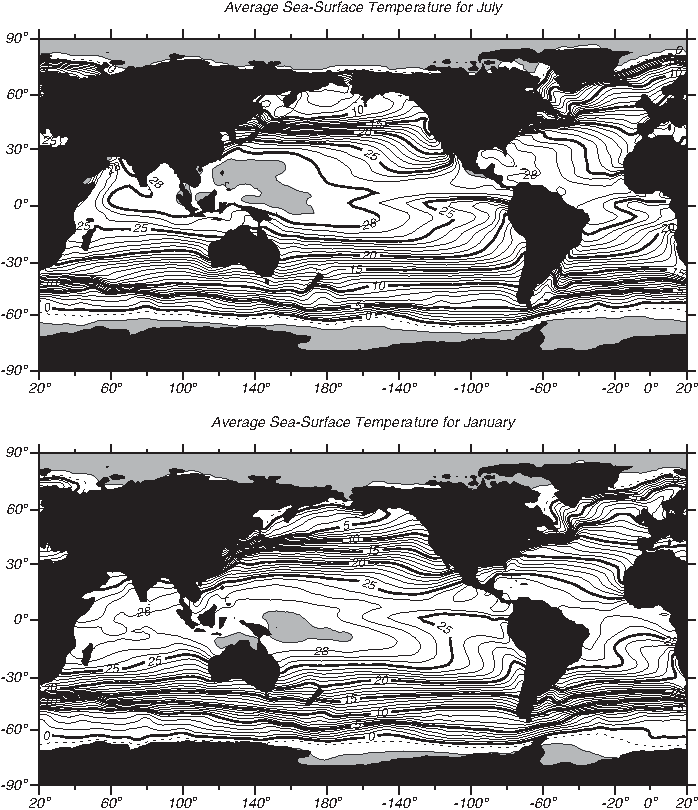
\includegraphics{sst_climatology} \footnotesize 
%% Figure 6.2 Mean sea-surface \rule{0mm}{3ex}temperature calculated from
%% the optimal interpolation technique (Reynolds and Smith, 1995) using
%% ship reports and \textsc{avhrr} measurements of temperature. Contour
%% interval is 1\degrees C with heavy contours every 5\degrees C. Shaded
%% areas exceed 29\degrees C.
%% \label{fig:sst_climatology}
%% \vspace{-4ex}
%% \end{figure}

Практическая шкала температуры изменялась в 1887, 1927, 1948, 1968 и
1990~гг., когда принимали всё более точные определения абсолютной
температуры. Наиболее современной является Международная температурная
шкала 1990~г. (МТШ-90). Она немного отличается от Международной практической
температурной шкалы 1968~г. (МПТШ-68). В точке $\degCent{0}$ они одинаковы, 
а выше неё МТШ-90 немного холоднее. Так, $t_{90}-t_{68} = -0.002$ 
при~$\degCent{10}$, $-0.005$ при~$\degCent{20}$, $-0.007$ при~$\degCent{30}$, 
и~$-0.010$ при~$\degCent{40}$. 
%% В оригинале отсутствует:
%% Отметим, что в то время, когда океанографы используют
%% термометры, калиброванные с точностью до миллиградуса ($\degCent{0.001}$), 
%% сама температурная шкала имеет недостоверность в несколько миллиградусов.
%
% The practical temperature scale was revised in 1887, 1927, 1948, 1968,
% and 1990 as more accurate determinations of absolute temperature
% became accepted. The most recent scale is the International
% Temperature Scale of 1990
% (\textsc{its}-90)\index{temperature!International Temperature
% Scale}. It differs slightly from the International Practical
% Temperature Scale of 1968 \textsc{ipts}-68. At 0\degrees C they are
% the same, and above 0\degrees C \textsc{its}-90 is slightly
% cooler. $t_{90}-t_{68} = -0.002$ at 10\degrees C, $-0.005$ at
% 20\degrees C, $-0.007$ at 30\degrees C and $-0.010$ at 40\degrees C.
%
%% \begin{figure}[b!]
%% \vspace{-3ex}
%% \makebox[121mm][c]{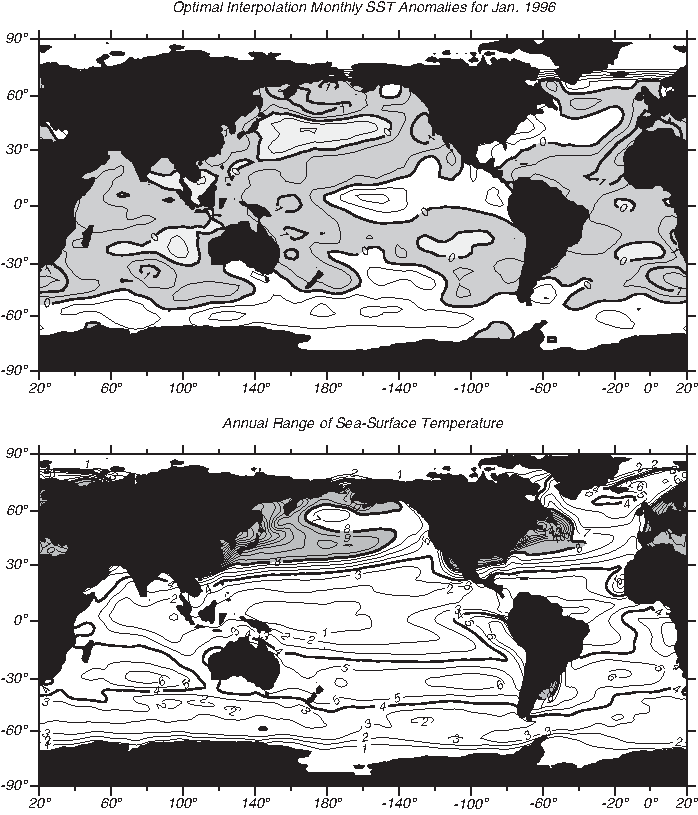
\includegraphics{SSTvariability}}
%% \footnotesize
%% Figure 6.3 \textbf{Top:} Sea-surface \rule{0mm}{3ex}temperature
%% anomaly for January 1996 relative to mean temperature shown in figure
%% 6.2 using data published by Reynolds and Smith (1995) in the
%% \textit{Climate Diagnostics Bulletin} for February 1995. Contour
%% interval is 1\degrees C. Shaded areas are
%% positive. \textbf{Bottom:}Annual range of sea-surface temperature in
%% \degrees{C} calculated from the Reynolds and Smith (1995) mean
%% sea-surface temperature data set. Contour interval is 1\degrees C with
%% heavy contours at 4\degrees C and 8\degrees C. Shaded areas exceed
%% 8\degrees C.
%% \label{fig:SSTvariability}
%% %\vspace{-3ex}
%% \end{figure}

% Notice that while oceanographers use thermometers calibrated with an
% accuracy\index{accuracy!temperature} of a millidegree, which is
% 0.001\degrees C, the temperature scale itself has uncertainties of a
% few millidegrees.
\end{section}

\begin{section}{Географическое распределение поверхностной температуры и солёности}
% \section[Geographical Distribution]{Geographical Distribution of Surface
% Temperature and Salinity}
Распределение поверхностной температуры моря стремится к \emph{зональному},
то есть, независимому от долготы (рис~6.2). Наиболее тёплые воды располагаются
вблизи экватора, наиболее холодные~--- у полюсов. Отклонения от зонального
распределения малы. По направлению от~\latlon{40}{N} к экватору, более
холодные воды стремятся к восточной части бассейна, а на север от этой
широты~--- к западной.
%
% \index{salinity!geographical distribution
% of}\index{temperature!geographical distribution of}The distribution of
% temperature at the sea surface tends to be \textit{zonal},
% \index{zonal|textbf}that is, it is independent of longitude (figure
% 6.2). Warmest water is near the equator, coldest water is near the
% poles. The deviations from zonal are small. Equatorward of 40\degrees,
% cooler waters tend to be on the eastern side of the basin. North of
% this latitude, cooler waters tend to be on the western side.

%% Рисунок 6.3 Средняя температура поверхности моря вычесленная с помощью
%% оптимальной интерполяционной техники (Reynolds and Smith, 1995) с
%% использованием данных корабельных наблюдений и измерений
%% AVHRR. Интервал между изолиниями~$\degCent{1}$, утолщённые изолинии через
%% каждые~$\degCent{5}$. Затенённые площади превышают~$\degCent{29}$.

\emph{Аномалии} температуры поверхности океана, то есть, отклонения от 
долгосрочного среднего, малы: они не превышают~$\degCent{1.5}$ (Harrison and Larkin, 1998), 
за исключением экваториальной зоны Тихого океана, где могут 
достигать~$\degCent{3}$ (рис.~6.3, верх).
%
% The \textit{anomalies} \index{anomalies!sea-surface
% temperature|textbf}of sea-surface temperature, the deviation from a
% long term average, are small, less than 1.5\degrees C (Harrison and
% Larkin, 1998) except in the equatorial Pacific where the deviations
% can be 3\degrees{C} (figure 6.3: top).
%
%% \begin{figure}[t!]
%% \makebox[121mm][c]{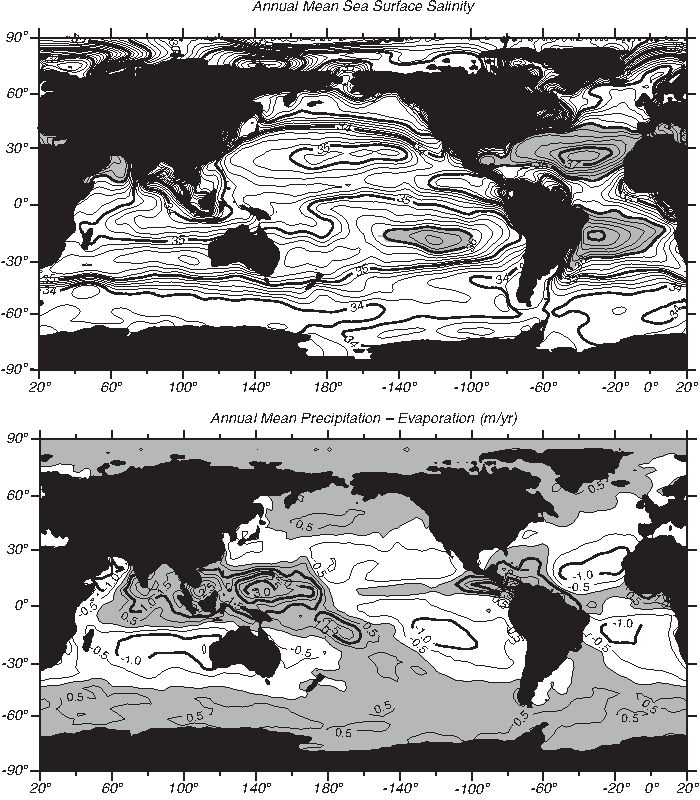
\includegraphics{salinity}}
%% \footnotesize
%% Figure 6.4 \textbf{Top}: Mean sea-surface \rule{0pt}{3ex}
%% salinity. \rule{0mm}{2ex}Contour interval is 0.25. Shaded areas exceed
%% a salinity of 36. From Levitus (1982).  \textbf{Bottom}: Precipitation
%% minus evaporation in meters per year calculated from global
%% rainfall\index{rainfall!global} by the Global Precipitation
%% Climatology Project and latent heat flux calculated by the Data
%% Assimilation Office, both at \textsc{nasa}'s Goddard Space Flight
%% Center. Precipitation exceeds evaporation in the shaded regions,
%% contour interval is 0.5 m.
%% 
%% \label{fig:salinity}
%% \vspace{-3ex}
%% \end{figure}

Годовая изменчивость поверхностной температуры максимальна в средних
широтах, особенно в западных частях океана (рис.~6.3, низ). На западе
зимой холодный воздух сдувается с континентов и охлаждает
океан, так что в тепловом балансе преобладает охлаждение. В тропиках
температурные изменения в большинстве своём не превышают~$\degCent{2}$.
%
% The annual range of surface temperature is highest at mid-latitudes,
% especially on the western side of the ocean (figure 6.3: bottom). In
% the west, cold air blows off the continents in winter and cools the
% ocean. The cooling dominates the heat budget. In the tropics the
% temperature range is mostly less than 2\degrees{C}.

Распределение поверхностной солёности также
стремится к зональному. Наиболее солёные воды~--- в средних широтах, где
велико испарение. Менее солёные воды находятся вблизи экватора, где их
опресняют выпадающие осадки, и в высоких широтах, где опреснение происходит 
вследствие таяния льда (рис.~6.4). Зональное среднее (восток-запад)
солёности демонстрирует хорошую корреляцию между солёностью и
испарением за вычетом осадков и с учетом речного стока (рис.~6.5).
%
% The distribution of sea-surface salinity also tends to be zonal. The
% saltiest waters are at mid-latitudes where evaporation is high. Less
% salty waters are near the equator where rain freshens the surface, and
% at high latitudes where melted sea ice freshens the surface (figure
% 6.4). The zonal (east-west) average of salinity shows a close
% correlation between salinity and evaporation minus precipitation plus
% river input (figure 6.5).

Если многие большие реки впадают в Атлантический и Северный Ледовитый океаны,
почему солёность Атлантики выше, чем Тихого океана? Брокер Broecker (1997) 
показал, что $0.32\Sv$~воды, испаряющейся над Атлантическим океаном, не
выпадает в виде осадков на сушу. Вместо этого она переносится ветрами в Тихий
океан (рис.~6.6). Брокер отмечает, что количество её невелико, лишь немного
больше, чем сток Амазонки, но <<пока этот поток не скомпенсируется
обменом более солёных Атлантических и менее солёных Тихоокеанских вод,
солёность внутренних частей Атлантики будет увеличиваться на~$1\gpl$
за тысячелетие>>.
%
% Because many large rivers drain into the Atlantic and the Arctic Sea,
% why is the Atlantic saltier than the Pacific? Broecker (1997) showed
% that 0.32 Sv of the water evaporated from the Atlantic does not fall
% as rain on land. Instead, it is carried by winds into the Pacific
% (figure 6.6). Broecker points out that the quantity is small,
% equivalent to a little more than the flow in the Amazon River, but
% ``were this flux not compensated by an exchange of more salty Atlantic
% waters for less salty Pacific waters, the salinity of the entire
% Atlantic would rise about 1 gram per liter per millennium.''

%% \begin{figure}[t!]
%% %\vspace{-2ex}
%% \makebox [121mm][c]{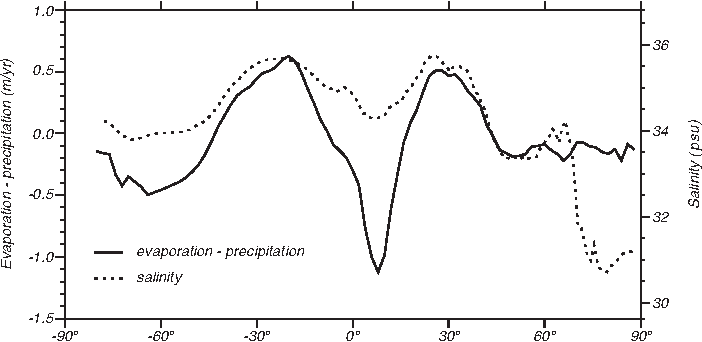
\includegraphics{zonalsalinity}}
%% \footnotesize
%% Figure 6.5 Zonal average of sea-surface \rule{0mm}{3ex}salinity
%% calculated for all the ocean from Levitus (1982) and the difference
%% between evaporation and precipitation ($E - P$) calculated from data
%% shown in figure 6.4 (bottom).
%% \label{fig:zonalsalinity}
%% \vspace{-5ex}
%% \end{figure}
%% 
%% \begin{figure}[b!]
%% \vspace{-3ex}
%% \makebox[121mm][c]{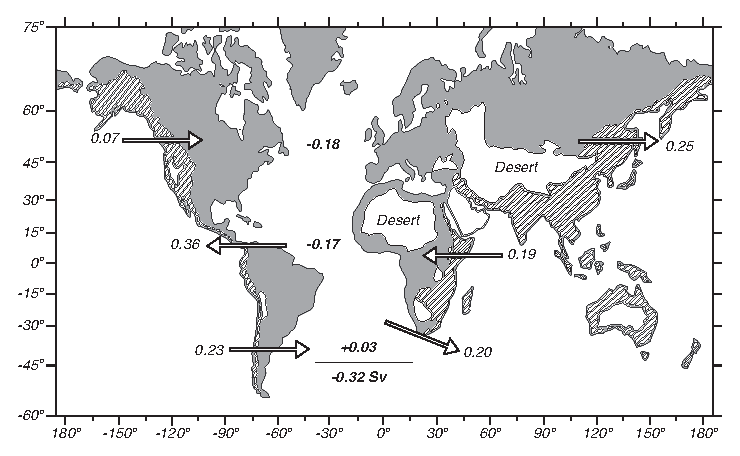
\includegraphics{BroeckerPlot}}
%% \footnotesize
%% Figure 6.6 Water \rule{0pt}{3ex} transported
%% \index{transport!atmospheric}by the atmosphere into and out of the
%% Atlantic. Basins draining into the Atlantic are black, deserts are
%% white, and other drainage basins are shaded. Arrows give direction of
%% water transport by the atmosphere, and values are in Sverdrups. Bold
%% numbers give the net transport for the Atlantic at each latitude
%% band. Overall, the Atlantic loses 0.32 Sv, an amount approximately
%% equal to the flow in the Amazon River. After Broecker (1997).
%% \label{fig:BroeckerPlot}
%% %\vspace{-4ex}
%% \end{figure}
%% 
%% \begin{figure}[t!]
%% %\vspace{-2ex}
%% \makebox[121 mm][c]{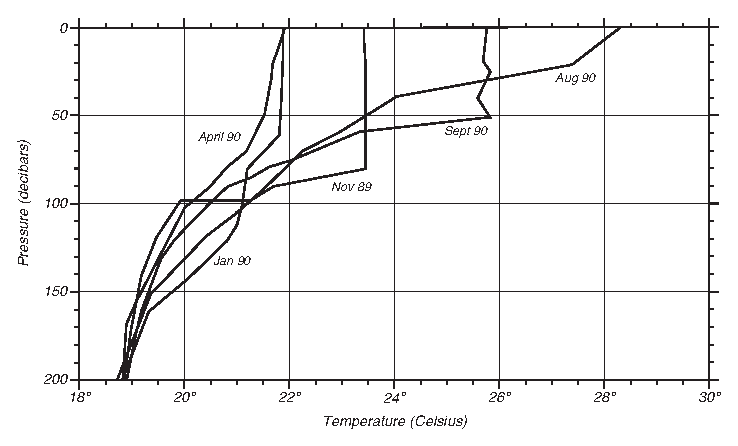
\includegraphics{seasonalthermo}}
%% \footnotesize
%% Figure 6.7 Growth and decay \rule{0mm}{4ex} of the mixed
%% layer\index{mixed layer!seasonal growth and decay} and seasonal
%% thermocline\index{thermocline!seasonal} from November 1989 to
%% September 1990 at the Bermuda Atlantic Time-series Station
%% (\textsc{bats}) at 31.8\degrees N 64.1\degrees W. Data were collected
%% by the Bermuda Biological Station for Research, Inc. Note that
%% pressure in decibars is nearly the same as depth in meters (see \S 6.8
%% for a definition of decibars).
%% \label{fig:seasonalthermo}
%% \vspace{-4ex}
%% \end{figure}

\begin{paragraph}{Средняя температура и солёность океана.} Средняя температура 
океана~$t=\degCent{3.5}$, а средняя солёность~$S=34.7$. Разброс вокруг среднего 
невелик: 50\% воды обладают следующими характеристиками:
\begin{align*}
\degCent{1.3} &< T < \degCent{3.8}\\ 
 34.6 &< S < 34.8
\end{align*}
%
% \textit{Mean Temperature and Salinity of the Ocean} \index{ocean!mean
% temperature|textbf}\index{ocean!mean salinity|textbf}The mean
% temperature of the ocean's waters is: t = 3.5\degrees{C}. The mean
% salinity is S = 34.7. The distribution about the mean is small: 50\%
% of the water is in the range:
% \begin{align}
% 1.3^{\circ}\text{C} < &\:t < 3.8^{\circ}\text{C} \notag \\
% 34.6 < &\:S < 34.8 \notag
% \end{align}
\end{paragraph}

%% Рисунок 6.4 Аномалии поверхностной температуры для Декабря 1995 года,
%% относительно средней температуры показанной на рисунке 6.3 на основе
%% данных опубликованных Reynolds and Smith (1995) в Climate Diagnostics
%% Bulletin за Февраль 1995. Интервал между изолиниями~$\degCent{1}$;
%% позитивные значения~--- затемнённые области.
%%
%% Рисунок 6.5 Годовые изменения температуры поверхности моря
%% в~$\degCent{}$ вычесленные по набору данных средних температур
%% поверхности моря Reynolds and Smith (1995). Интервал между
%% изолиниями~$\degCent{1}$, утолщённые изолинии через
%% каждые~$\degCent{4}$ и~$\degCent{8}$. Затенённые площади
%% превышают~$\degCent{29}$.
%%
%% Рисунок 6.6 Средняя солёность поверхности моря. Изолинии проведены
%% через 0.25 п.е.с. Затенённые площади превышают 36 п.е.с. (Взято из
%% Levitus, 1982).
%% 
%% Рисунок 6.7 Зональное среднее для поверхностной солёности расчитанное
%% для всех океанов из Levitus (1982) и разница между испарением и
%% осадками (E-P) расчитанная по данным представленным на Рисунке 5.14.
%%
%% Рисунок 6.8 Вода перемещаемая атмосферой в Атлантику и из
%% Атлантики. Бассейны стекающие в Атлантику изображены чёрным, пустыни
%% белым, а бруги дренажные бассейны затенены. Стрелочками показаны
%% направления транспорта воды атмосферой и его значения в
%% Свердрупах. Цифры выделенные жирным шрифтом~--- чистый транспорт для
%% Атлантики. В целом Атлантика теряет 0,32 Св, объём сопоставимый со
%% стоком Амазонки. Взято из Broecker (1997).
\end{section}

\begin{section}{Перемешанный слой в океане}
% \section{The Oceanic Mixed Layer and Thermocline}
Ветер, дующий над океаном, воздействует на его верхние слои, приводя к 
образованию тонкого \emph{перемешанного слоя}, имеющего постоянную температуру
и солёность от поверхности до глубины, где их значения отличаются от
поверхностных. Величина этой разницы выбирается произвольно, но как правило,
температура на нижней границе слоя должна быть не более чем 
на $0.02$--$\degCent{0.1}$ холоднее, чем на поверхности. Отметим, что 
и температура, и солёность в этом слое должны быть постоянны. Позже мы увидим, 
что средняя скорость (???чего) в перемешанном слое может изменяться.
%% в первоначальном переводе добавлено: "изменяться [с глубиной]".
Типичная толщина перемешанного слоя в тропических и средних широтах
составляет около~$10$--$200\m$.
%
% Wind blowing on the ocean stirs the upper layers leading to a thin
% \textit{mixed layer} \index{mixed layer|textbf}at the sea surface
% having constant temperature and salinity from the surface down to a
% depth where the values differ from those at the surface. The magnitude
% of the difference is arbitrary, but typically the temperature at the
% bottom of the layer must be no more than 0.02--0.1\degrees\ colder
% than at the surface. Note that both temperature and salinity must be
% constant in the mixed layer. We will see later that mean velocity is
% not constant. The mixed layer is roughly 10--200 m thick over most of
% the tropical and mid-latitude belts.


Глубина и температура перемешанного слоя изменяется с каждым днем и от
от сезона к сезону под воздействием двух процессов:
%
% The depth and temperature of the mixed layer\index{mixed
% layer!external forcing of} varies from day to day and from season to
% season in response to two processes:
\begin{enumerate}
\item
Потоки тепла через поверхность нагревают и охлаждают поверхностную
воду. Изменения температуры влияют на контраст плотности между
перемешанным слоем и подстилающими водами. Чем сильнее контраст, тем
большая работа требуется, чтобы перемешать слой в вертикальном
направлении.
%
% \vitem 
% Heat fluxes through the surface heat and cool the surface
% waters. Changes in temperature change the density contrast between the
% mixed layer and deeper waters. The greater the contrast, the more work
% is needed to mix the layer downward and visa versa.

\item
Турбулентность в перемешанном слое, которая зависит от скорости ветра 
и интенсивности обрушения волн, обеспечивает механическую работу,
необходимую для транспортировки тепла вниз. Turbulence mixes water in the
layer, and it mixes the water in the layer with water in the thermocline.
% 
% \vitem 
% Turbulence in the mixed layer mixes heat downward. The
% turbulence\index{turbulence!in mixed layer} depends on the wind speed
% and on the intensity of breaking waves. Turbulence mixes water in the
% layer, and it mixes the water in the layer with water in the
% thermocline\index{thermocline}.
\end{enumerate}

В средних широтах толщина перемешанного слоя минимальна поздним летом, 
когда ветры слабы, а солнечный свет хорошо прогревает поверхностный
слой (рис.~6.7). Временами прогрев настолько велик, а ветры настолько слабы, 
что толщина перемешанного слоя уменьшается до нескольких метров. Осенью ранние
штормы переносят тепло в более глубокие слои, увеличивая толщину
перемешанного слоя, но часть тепла при этом теряется. Зимой тепло
уходит, и перемешанный слой продолжает увеличиваться, достигая
максимума поздней зимой. Весной ветры ослабевают, поступление
солнечного света увеличивается, и формируется новый перемешанный слой.
%
% The mid-latitude mixed layer\index{mixed layer!mid-latitude} is
% thinnest in late summer when winds are weak, and sunlight warms the
% surface layer (figure 6.7). At times, the heating is so strong, and
% the winds so weak, that the layer is only a few meters thick. In fall,
% the first storms of the season mix the heat down into the ocean
% thickening the mixed layer, but little heat is lost. In winter, heat
% is lost, and the mixed layer continues to thicken, becoming thickest
% in late winter. In spring, winds weaken, sunlight increases, and a new
% mixed layer forms.

%% \begin{figure}[t!]
%% %\vspace{-2ex}
%% \makebox[121 mm] [c] {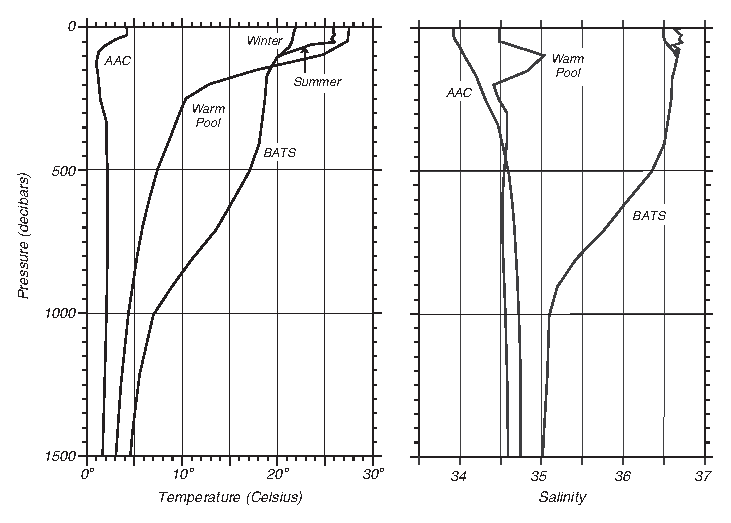
\includegraphics{TandSProfile}}
%% %\centering
%% \footnotesize
%% Figure 6.8 Typical \rule{0mm}{4ex}temperature and salinity profiles in
%% the open ocean. AAC: At 62.0\degrees\ S, 170.0\degrees\ E in the
%% Antarctic Circumpolar Current\index{Antarctic Circumpolar Current} on
%% 16 January 1969 as measured by the \textit{R/V Hakuho Maru}. Warm
%% Pool: At 9.5\degrees\ N 176.3\degrees\ E in the tropical west Pacific
%% warm pool on 12 March 1989 as measured by Bryden and Hall on the
%% \textit{R/V Moana Wave}.  \textsc{bats}: At 31.8\degrees\ N
%% 64.1\degrees\ W near Bermuda on 17 April and 10 September 1990 as
%% measured by the Bermuda Biological Station for Research, Inc.  Data
%% are included with Java OceanAtlas.
%% \label{fig:TandSProfile}
%% \vspace{-5ex}
%% \end{figure}

%% (Рисунок 6.9 верхняя часть). Он часто более
%% солёный чем подстилающие воды (исключение в этом смысле составляют
%% высокие широты) (Рисунок 6.9 нижняя часть). 

Температура воды под перемешанным слоем быстро убывает с глубиной, за 
исключением высоких широт. Диапазон глубин, в котором скорость изменений
(градиент температуры) максимальна, называется \emph{термоклином}. 
Так как плотность тесно связана с температурой, термоклин чаще всего 
совпадает с \emph{пикноклином}~--- слоем, обладающим наибольшим градиентом
плотности.
%
% Below the mixed layer\index{mixed layer!mid-latitude}, water
% temperature decreases rapidly with depth except at high latitudes. The
% range of depths where the rate of change, the gradient of temperature,
% is large is called the
% \textit{thermocline}\index{thermocline|textbf}. Because density is
% closely related to temperature, the thermocline also tends to be the
% layer where density gradient is greatest, the
% \textit{pycnocline}\index{pycnocline|textbf}.

Если форма термоклина подвержена существенным сезонным изменениям (рис.~6.7),
то его принято называть \emph{сезонным термоклином}. Наряду с ним 
существует \emph{постоянный термоклин}, который расположен ниже сезонного и 
простирается до глубины~$1500$--$2000\m$ (рис.~6.8). В высоких широтах, 
например, в таких, где расположена показанная на рисунке станция~AAC, 
над постоянным термоклином может располагаться слой более холодной 
и менее солёной воды.
%
% The shape of the thermocline varies slightly with the seasons (figure
% 6.7). This is the \textit{seasonal thermocline}.
% \index{thermocline!seasonal|textbf} The \textit{permanent thermocline}
% \index{thermocline!permanent|textbf}extends from below the seasonal
% thermocline to depths of 1500--2000 meters (figure 6.8). At high
% latitudes, such as at the \textsc{aac} station in the figure, there
% may be a cooler, fresher layer above the permanent thermocline.

Солёность перемешанного слоя имеет тенденцию превышать солёность термоклина
в области $\degrees{10}$--$\degrees{40}$~широты, где испарение с поверхности
океана превышает объем осадков. В более высоких широтах перемешанный слой
более пресный, так как выпадение осадков и таяние льда уменьшают солёность.
В некоторых тропических регионах, таких как warm pool in the western 
tropical Pacific, благодаря осадкам также образуется тонкий распресненный
перемешанный слой.
%
% The mixed layer tends to be saltier than the
% thermocline\index{thermocline} between 10\degrees\ and 40\degrees\
% latitude, where evaporation exceeds precipitation. At high latitudes
% the mixed layer\index{mixed layer!high latitude} is fresher because
% rain and melting ice reduce salinity. In some tropical regions, such
% as the warm pool in the western tropical Pacific, rain also produces a
% thin fresher mixed layer\index{mixed layer!tropical Pacific}.

%% Figure 6.7 Growth and decay of the mixed layer and seasonal
%% thermocline from November 1989 to September 1990 at the Bermuda
%% Atlantic Time-series Station (BATS) at \latlon{31.8}{N}
%% \latlon{64.1}{W}. Data were collected by the Bermuda Biological
%% Station for Research, Inc. Note that pressure in decibars is nearly
%% the same as depth in meters (see \S~6.8 for a definition of decibars).

%% Figure 6.8 Typical temperature and salinity profiles in the open
%% ocean. AAC: At \latlon{62.0}{S}, \latlon{170.0}{E} in the Antarctic
%% Circumpolar Current on 16 January 1969 as measured by the R / V Hakuho
%% Maru. Warm Pool: At \latlon{9.5}{N}\latlon{176.3}{E} in the tropical
%% west Pacific warm pool on 12 March 1989 as measured by Bryden and Hall
%% on the R / V Moana Wave. BATS: At \latlon{31.8}{N} \latlon{64.1}{W}
%% near Bermuda on 17 April and 10 September 1990 as measured by the
%% Bermuda Biological Station for Research, Inc. Data are included with
%% Java Ocean Atlas.
\end{section}

\begin{section}{Плотность, потенциальная температура и нейтральная плотность}
% \section[Density]{Density, Potential Temperature, and Neutral Density}
Холодная вода, которая образуется на поверхности океана в зимний период,
погружается на глубину, зависящую от плотности глубинной воды. Далее вода
переносится течениями в другие части океана. В целом, частица воды 
перемещается таким образом, чтобы оставаться на линии раздела между 
менее плотной и более плотной водой. Распределение течений в океане зависит 
от распределения давления, которое, в свою очередь, зависит от изменчивости
плотности океанической воды, как это кратко рассмотрено в разд.~\ref{sec:10.4}.
Таким образом, если мы желаем проследить перемещение воды в океане, нам
потребуется знать, как в океане распределена плотность.
%
% During winter, cold water formed at the surface sinks to a depth
% determined by its density relative to the density of the deeper
% water. Currents then carry the water to other parts of the ocean. At
% all times, the water parcel moves to stay below less dense water and
% above more dense water. The distribution of currents within the ocean
% depends on the distribution of pressure, which depends on the
% variations of density inside the ocean as outlined in \S10.4. So, if
% we want to follow water movement within the ocean, we need to know the
% distribution of density within the ocean.

\begin{paragraph}{Плотность и~$\sigma_t$.}
% \paragraph{Density and sigma-t}
Вычисление перемещений воды требует измерения плотности с точностью до 
нескольких частей на миллион, что является трудной задачей.
%
% \index{density}The calculation of water movement requires measurements
% of density with an accuracy\index{accuracy!density} of a few parts per
% million. This is not easy.

\emph{Абсолютную плотность} воды возможно измерить только в специализированых 
лабораториях, причем даже там этот процесс сопряжен с определенными 
трудностями. Наилучшая точность составляет $1:2.5\times 10^5 = 4$~части 
на миллион. 
%
% \textit{Absolute Density} \index{density!absolute|textbf}of water can
% only be measured in special laboratories, and only with
% difficulty. The best accuracy is $1\,:\, 2.5 \times 10^5 = 4$ parts
% per million.

Чтобы избежать сложностей работы с абсолютной
плотностью, океанографы используют плотность, относительную к плотности
чистой воды. Плотность~$\rho(S,t,p)$ теперь определяют, используя
Стандартную среднюю океанскую воду, которая имеет известный изотопный состав
и считается насыщенной растворёнными атмосферными газами. Здесь $S$,
$t$, $p$~--- солёность, температура и давление соответственно.
%
% To avoid the difficulty of working with absolute density,
% oceanographers use density relative to density of pure water. Density
% $\rho (S, t, p)$ is now defined using Standard Mean Ocean Water of
% known isotopic composition, assuming saturation of dissolved
% atmospheric gasses. Here $S, t, p$ refers to salinity, temperature,
% and pressure.

%% Figure 6.9 Profiles of Left in situ and potential temperature and
%% Right sigma-t and sigma-theta in the Kermadec Trench in the Pacific
%% measured by the R / V Eltanin during the Scorpio Expedition on 13 July
%% 1967 at \latlon{175.825}{E} and \latlon{28.258}{S}. Data from Warren
%% (1973).

На практике измерения плотности не проводятся, она вычисляется на основе
измеренных \emph{in situ} давления, температуры и электропроводности согласно
уравнению состояния морской воды. Точность этого метода составляет две части
на миллион.
%
% In practice, density is not measured, it is calculated from \textit{in
% situ} \index{in situ} measurements of pressure, temperature, and
% conductivity using the equation of state for sea water. This can be
% done with an accuracy\index{accuracy!density} of two parts per
% million.

Плотность воды на поверхности обычно составляет~$1027\kgpcm$. В работах по
физике океана часто ограничиваются для простоты двумя последними
цифрами плотности, и эту величину называют \emph{аномалией плотности}:
\begin{equation}
 \sigma(s,t,p) = \rho(s,t,p)-1000\kgpcm.
\end{equation}
Рабочая группа МАФНО по единицам измерений, терминологии и обозначениям 
в океанологии рекомендовала (SUN, 1985) заменить~$\sigma$ буквой~$\gamma$, 
так как величина~$\sigma$ изначально определялась относительно чистой воды 
и была безразмерной. Однако, в данном пособии мы будем следовать устоявшейся 
практике и использовать обозначение~$\sigma$.
%
% Density of water at the sea surface is typically 1027 kg/m$^3$. For
% simplification, physical oceanographers often quote only the last 2
% digits of the density, a quantity they call \textit{density anomaly}
% or \textit{Sigma (S,t,p)}\index{density!anomaly or sigma|textbf}:
% \begin{equation}
% \sigma(S,t,p) = \rho (S, t, p) - 1000 \text{\ kg/m$^3$}
% \end{equation}
% The Working Group on Symbols, Units and Nomenclature in Physical
% Oceanography (\textsc{sun}, 1985) recommends that $\sigma$ be replaced
% by $\gamma$ because $\sigma$ was originally defined relative to pure
% water and it was dimensionless. Here, however, I will follow common
% practice and use $\sigma$.

В ходе изучения поверхностных слоёв океана сжимаемостью воды можно пренебречь
и ввести новую величину~$\sigma_t$:
\begin{equation}\label{eq:6.8}
\sigma_t = \sigma(S,t,0). 
\end{equation}
Это аномалия плотности воды, когда всё давление на нее полагается равным
атмосферному (т.~е.\ нулевому давлению воды), а температура и солёность 
обладают значениями, измеренными \emph{in situ}.
%
% If we are studying surface layers of the ocean, we can ignore
% compressibility, and we use a new quantity sigma-t (written $\sigma_t$):
% \begin{equation}
% \sigma _t =  \sigma(S,t,0)
% \end{equation}
% This is the density anomaly of a water sample when the total pressure
% on it has been reduced to atmospheric pressure (\textit{i.e.} zero
% water pressure), but the temperature and salinity are \textit{in situ}
% values.\index{in situ}
%
%% \begin{figure}[t!]
%% \makebox[121 mm] [c] {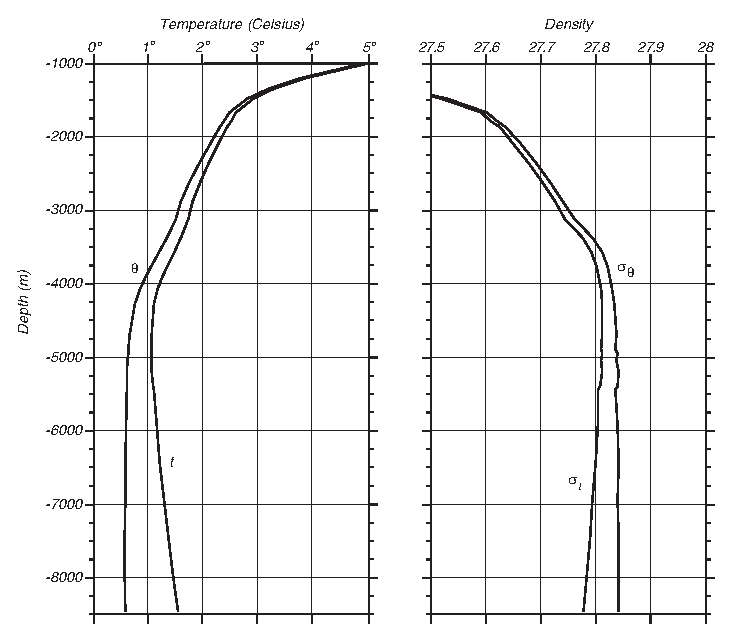
\includegraphics{thetaprofile}}
%% \footnotesize
%% Figure 6.9 Profiles \rule{0mm}{4ex}of \textbf{Left} \textit{in
%% situ}\index{in situ} $t$ and potential $\theta$ temperature and
%% \textbf{Right} sigma-t and sigma-theta in the Kermadec Trench in the
%% Pacific measured by the R/V Eltanin during the Scorpio Expedition on
%% 13 July 1967 at 175.825\degrees\ E and 28.258\degrees\ S. Data from
%% Warren (1973).
%% 
%% \label{fig:thetaprofile}
%% \vspace{-4ex}
%% \end{figure}
\end{paragraph}

\begin{paragraph}{Потенциальная температура.}
% \paragraph{Potential Temperature}
Если частица воды перемещается в океане глубже перемешанного слоя, её 
солёность и температура может изменяться исключительно в ходе смешивания с 
другой водой. Следовательно, мы можем воспользоваться измеренными значениями
температуры и солёности для определения пути движения воды. Лучше всего это
удается сделать, если предварительно компенсировать влияние сжимаемости воды.
%
% \index{temperature!potential}\index{potential!temperature}As a water
% parcel moves within the ocean below the mixed layer\index{mixed
% layer}, its salt and heat content can change only by mixing with other
% water. Thus we can use measurements of temperature and salinity to
% trace the path of the water. This is best done if we remove the effect
% of compressibility.

Когда вода погружается в глубины океана, давление увеличивается, 
вода сжимается, и сжатие совершает над ней работу. При этом внутренняя 
энергия воды увеличивается. Чтобы представить себе, как это происходит, 
рассмотрим куб с определённой массой воды внутри. Когда куб погружается, 
его стороны начинают прогибаться внутрь, так как куб сжимается. Напомним, что
работа~--- это сила, умноженная на расстояние, а значит, работа~--- это 
расстояние, на которое погрузилась сторона куба, умноженное на силу, 
приложенную к этой стороне давлением. Изменение внутренней энергии может
как вызвать, так и не вызвать изменение температуры (McDougall and Feistel, 2003).
Внутренняя энергия жидкости представляет собой сумму молекулярной кинетической
энергии (температура) и молекулярной потенциальной энергии. В морской воде
преобладает последняя, а изменение внутренней энергии ведет к изменению
температуры, показанному на рис.~6.9. На глубине~$8\km$ увеличение температуры
составляет почти~$\degCent{0.9}$.
%
% As water sinks, pressure increases, the water is compressed, and the
% compression does work on the water. This increases the internal energy
% of the water. To understand how compression increases energy, consider
% a cube containing a fixed mass of water. As the cube sinks, its sides
% move inward as the cube is compressed. Recalling that work is force
% times distance, the work is the distance the side moves times the
% force exerted on the side by pressure. The change in internal energy
% may or may not result in a change in temperature (McDougall and
% Feistel, 2003). The internal energy of a fluid is the sum of molecular
% kinetic energy (temperature) and molecular potential energy. In sea
% water, the later term dominates, and the change of internal energy
% produces the temperature change shown in figure 6.9. At a depth of 8
% km, the increase in temperature is almost 0.9\degrees\ C.

Чтобы устранить влияние сжимаемости на процесс измерения температуры,
океанографы (и метеорологи, которые сталкиваются с такой же проблемой 
в атмосфере) используют концепцию потенциальной температуры. 
\emph{Потенциальная температура}~$\Theta$~--- это температура частицы воды
на поверхности моря, поднятой адиабатически с глубины к
поверхности океана. Поднять частицу \emph{адиабатически} значит поднять её 
будто в изолированном контейнере, без теплообмена с окружающей средой.
На практике, безусловно, никто воду на поверхность не поднимает. 
Потенциальная температура рассчитывается по температуре воды на глубине.
%
% To remove the influence of compressibility from measurements of
% temperature, oceanographers (and meteorologists who have the same
% problem in the atmosphere) use the concept of potential
% temperature. \textit{Potential temperature}
% \index{temperature!potential|textbf}\index{potential!temperature|textbf}
% $\Theta$ is defined as the temperature of a parcel of water at the sea
% surface after it has been raised adiabatically from some depth in the
% ocean. Raising the parcel \textit{adiabatically}
% \index{adiabatically|textbf}means that it is raised in an insulated
% container so it does not exchange heat with its surroundings. Of
% course, the parcel is not actually brought to the surface. Potential
% temperature is calculated from the temperature in the water at depth,
% the \textit{in situ}\index{in situ} temperature.
\end{paragraph}

\begin{paragraph}{Потенциальная плотность.}
% \paragraph{Potential Density}
При изучении промежуточных водных слоев океана (например, на глубинах 
порядка~$1\km$) уже невозможно игнорировать сжимаемость. Так как изменение 
давления влияет, в основном, на температуру воды, это влияние в первом 
приближении может быть устранено введением понятия
\emph{потенциальной плотности}.
%
% \index{density!potential|textbf}\index{potential!density|textbf}If we
% are studying intermediate layers of the ocean, say at depths near a
% kilometer, we cannot ignore compressibility. Because changes in
% pressure primarily influence the temperature of the water, the
% influence of pressure can be removed, to a first approximation, by
% using the \textit{potential density}.

\emph{Потенциальная плотность}~$\rho _{\Theta}$~--- это плотность частицы 
воды, которую она бы имела, если бы была поднята на поверхность адиабатически 
и без изменения солёности. Аномалия потенциальной плотности такой частицы, 
\begin{equation}\label{eq:6.9}
\sigma_\Theta = \sigma(S,\Theta,0),
\end{equation}
особенно полезна, поскольку представляет собой сохраняющееся термодинамическое 
свойство.
%% В оригинале отсутствует:
%% Потенциальная плотность используется так как устраняет основное
%% влияние давления на плотность. Она позволяет нам сравнивать плотность
%% проб морской воды с разных глубин. Также она используется потому что
%% вода течёт вдоль поверхностей постоянной потенциальной плотности.
%
% \textit{Potential density} $\rho _{\Theta}$ is the density a parcel of
% water would have if it were raised adiabatically to the surface
% without change in salinity. Written as sigma,
% \begin{equation}
% \sigma _{\Theta} = \sigma(S, \Theta, 0)
% \end{equation}
% $\sigma _{\Theta}$ is especially useful because it is a conserved
% thermodynamic property.

Потенциальная плотность непригодна при сравнении плотности воды на очень
больших глубинах. Если мы поднимем две частицы воды на поверхность и сравним
их плотности, то в процессе вычисления потенциальной плотности не будет учтено
влияние давления на коэффициенты теплового и salt расширения. В результате,
две пробы воды, взятые с глубины~$4\km$, с одинаковой плотностью, но различной 
температурой и солёностью, могут иметь существенно различную потенциальную
плотность. В некоторых регионах использование~$\rho(\Theta)$ может показать
мнимое уменьшение плотности с глубиной (рис.~6.10), в то время как нам 
известно, что это невозможно, поскольку такой столб воды был бы нестабилен.
%
% Potential density is not useful for comparing density of water at
% great depths. If we bring water parcels to the surface and compare
% their densities, the calculation of potential density ignores the
% effect of pressure on the coefficients for thermal and salt
% expansion. As a result, two water samples having the same density but
% different temperature and salinity at a depth of four kilometers can
% have noticeably different potential density. In some regions the use
% of $\rho(\Theta)$ can lead to an apparent decrease of density with
% depth (figure 6.10) although we know that this is not possible because
% such a column of water would be unstable.

%% \begin{figure}[b!]
%% \vspace{-2ex}
%% 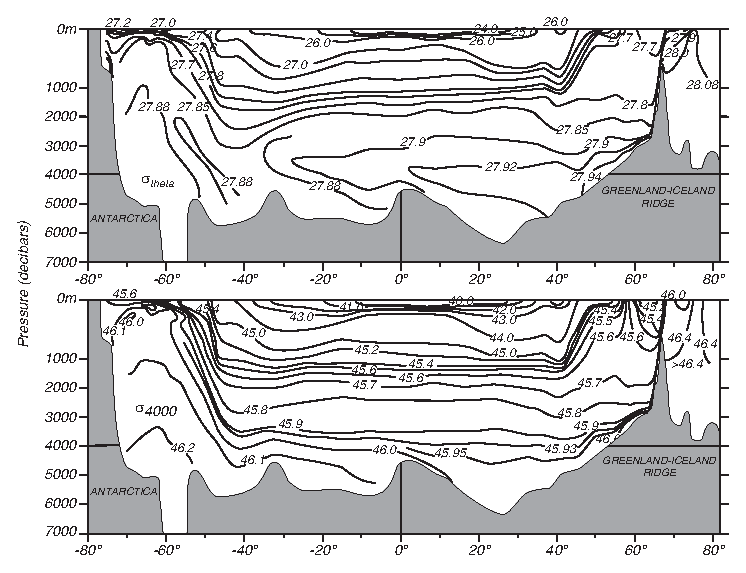
\includegraphics{atlsection}
%% \footnotesize
%% Figure 6.10 Vertical \rule{0mm}{4ex}sections of density in the western
%% Atlantic.  Note that the depth scale changes at 1000 m
%% depth. \textbf{Upper}: $\sigma _{\Theta}$, showing an apparent density
%% inversion below 3,000 m. \textbf{Lower}: $\sigma _4$ showing
%% continuous increase in density with depth. After Lynn and Reid (1968).
%% \label{fig:atlsection4}
%% %\vspace{-4ex}
%% \end{figure}

При сравнении проб с больших глубин, более корректный подход состоит в 
использовании аномалий плотности, вычисленных не на поверхности ($p = 0$), 
а на определенной глубине, достаточно близкой к исследуемой. Например, мы
можем рассмотреть пробы под давлением~$4\,000\dBar$, приближенно 
соответствующим глубине в~$4\km$:
\begin{equation}\label{eq:6.10}
\sigma_4 = \sigma(S, \Theta, 4000),
\end{equation}
где $\sigma_4$~--- плотность частицы воды, погружённой адиабатически на
глубину, соответствующую давлению~$4\,000\dBar$. В более общем случае,
иногда используется~$\rho_r$:
\begin{equation}
 \sigma_r = \sigma(S, \Theta, p, p_r),
\end{equation}
где~$p$~--- давление, а $p_r$~--- давление на некоторой заданной глубине.
В формулах~(\ref{eq:6.8}) и~(\ref{eq:6.10}) $p_r = 0\dBar$ и~$p_r = 4000\dBar$
соответственно. 
%% нестыковка: 
%%
%% 1) $\rho_r$ возникает ниоткуда и более не используется. Возможно,
%%    надо добавить связку: "плотность $\rho_r$. аномалия которой
%%
%% 2) \sigma(S, \Theta, p, p_r) --- откуда там 4 параметра вместо 3-х?
%%    возможно, там "p - p_r" --- т.е. перепад давления?
%%
%% 3) вместо упомянутой формулы (6.9) уместнее (6.10)
%
% To compare samples from great depths, it is better to bring both
% samples to a nearby depth instead of to the surface $p = 0$. For
% example, we can bring both parcels to a pressure of 4,000 decibars,
% which is near a depth of 4 km:
% \begin{equation}
% \sigma_4 = \sigma(S, \Theta, 4000)
% \end{equation}
% where $\sigma_4$ is the density of a parcel of water brought
% adiabatically to a pressure of 4,000 decibars. More generally,
% oceanographers sometimes use $\rho_r$
% \begin{equation}
% \sigma _r = \sigma(S, \Theta, p, p_r)
% \end{equation}
% where $p$ is pressure, and $p_r$ is pressure at some reference
% level. In (6.8) the level is $p_r = 0$ decibars, and in (6.9) $p_r =
% 4000$ decibars.


Применение~$\sigma_r$ порождает определенные проблемы. Если нам требуется
проследить путь некоторой частицы воды в глубинах океана, то в некоторых 
регионах придется воспользоваться, к примеру, величиной~$\sigma_3$, а в
других~--- $\sigma_4$. Но что происходит, когда частица воды перемещается
с глубины~$3\km$ в одном регионе на глубину~$4\km$ в другом? При переходе
от~$\sigma_3$ к~$\sigma_4$ в функции плотности возникает разрыв. Чтобы
устранить это затруднение, Джекет и Мак-Дугалл Jackett and McDougall (1997)
ввели новую величину, которую назвали нейтральной плотностью. 
%
% The use of $\sigma_r$ leads to problems. If we wish to follow parcels
% of water deep in the ocean, we might use $\sigma_3$ in some areas, and
% $\sigma_4$ in others.  But what happens when a parcel moves from a
% depth of 3 km in one area to a depth of 4 km in another? There is a
% small discontinuity between the density of the parcel expressed as
% $\sigma_3$ compared with density expressed as $\sigma_4$. To avoid
% this difficulty, Jackett and McDougall (1997) proposed a new variable
% they called neutral density.

%% Figure 6.12 Вертикальный разрез солёности в западной
%% Атлантике. Масштаб глубины изменяется на 1000 м. Гидрографические
%% станции помечены точками. Верхний: Сигма-$\Theta$, демонстрирует
%% мнимую инверсию плотности ниже 3000. Нижний: Сигма(4) демонстрирует
%% плавное увеличение плотности с глубиной. Взято из Lynn and Reid, 1968.
\end{paragraph}

\begin{paragraph}{Нейтральные поверхности и плотность.}
% \paragraph{Neutral Surfaces and Density}
Частица воды перемещается по траектории, сохраняющей плотность неизменной,
поэтому её путь лежит между менее плотной водой сверху и более плотной~--- 
снизу. В более точной формулировке, перемещение происходит по линии постоянной
потенциальной плотности~$\sigma_r$ на текущей глубине~$r$. Эта линия получила
название~\emph{нейтрального пути} (Eden and Willebrand, 1999). 
A \emph{neutral surface element} is the surface tangent to the neutral paths 
through a point in the water. При перемещении частицы воды по этой поверхности
не совершается никакой работы, поскольку отсутствуют (если пренебречь трением)
силы плавучести, воздействующие на частицу во время её движения.
%
% \index{neutral surfaces}\index{density!neutral surfaces}A parcel of
% water moves locally along a path of constant density so that it is
% always below less dense water and above more dense water. More
% precisely, it moves along a path of constant potential density
% $\sigma_r$ referenced to the local depth $r$. Such a path is called a
% \textit{neutral path}\index{neutral path|textbf} (Eden and Willebrand,
% 1999). A \textit{neutral surface element} \index{neutral surface
% element|textbf}is the surface tangent to the neutral paths through a
% point in the water. No work is required to move a parcel on this
% surface because there is no buoyancy\index{buoyancy} force acting on
% the parcel as it moves (if we ignore friction).

%
% Now let's follow the parcel as it moves away from a local region. At
% first we might think that because we know the tangents to the surface
% everywhere, we can define a surface that is the envelope of the
% tangents. But an exact surface is not mathematically possible in the
% real ocean, although we can come very close.

Джекет и Мак-Дугалл предложили Jackett and McDougall (1997) практически
пригодное определение нейтральной плотности~$\gamma^n$ и поверхности,
которая приближенно равна идеальной с разницей порядка нескольких десятков 
метров в любой точке океана. Этот результат был получен на основе данных
из атласа Levitus (1982). Величины нейтральной плотности, в свою очередь,
были в дальнейшем использованы to label the data in the Levitus atlas.
Этот prelabeled data set применяется при вычислении~$\gamma^n$ в новых
точках, в которых $t$ и~$S$ представляются в виде функции глубины путем
интерполяции по четырем ближайшим точкам, входящим в атлас. Благодаря этому
подходу, нейтральная плотность~$\gamma^n$ определяется как функция 
\emph{in situ}-значений солёности~$S$ и температуры~$t$, а также давления~$p$,
широты и долготы.
%
% Jackett and McDougall (1997) developed a practical neutral density
% variable $\gamma^n$ and surface that stays within a few tens meters of
% an ideal surface anywhere in the world.  They constructed their
% variables using data in the Levitus (1982) atlas. The neutral density
% values were then used to label the data in the Levitus atlas. This
% prelabeled data set is used to calculate $\gamma^n$ at new locations
% where $t, S$ are measured as a function of depth by interpolation to
% the four closest points in the Levitus atlas. Through this practice,
% neutral density $\gamma^n$ is a function of salinity $S$, \textit{in
% situ}\index{in situ} temperature $t$, pressure $p$, longitude, and
% latitude.

Нейтральная поверхность, определенная выше, отличается от идеальной 
незначительно. Так, если частица воды вовлечена в круговую циркуляцию 
%% "круговая циркуляция" == gyre???
по нейтральной поверхности, ее итоговая глубина будет отличаться от начальной 
примерно на~$10\m$. С другой стороны, при использовании поверхностей
потенциальной плотности, разница может составить сотни метров~--- гораздо 
большую погрешность.
%
% The neutral surface defined above differs only slightly from an ideal
% neutral surface. If a parcel moves around a gyre on the neutral
% surface and returns to its starting location, its depth at the end
% will differ by around 10 meters from the depth at the start. If
% potential density surfaces are used, the difference can be hundreds of
% meters, a far larger error.
\end{paragraph}

\begin{paragraph}{Уравнение состояния морской воды.}
% \paragraph{Equation of state of sea water}
Плотность морской воды измеряется редко. \emph{Плотность рассчитывается по
измерениям температуры, электропроводности или солёности и давления с
помощью уравнения состояния морской воды.} \emph{Уравнение состояния} морской
воды~--- это уравнение, которое связывает плотность с температурой,
солёностью и давлением.
%
% \index{density!equation!of state|textbf}\index{equation of
% state|textbf}Density of sea water is rarely measured.  \textit{Density
% is calculated from measurements of temperature, conductivity, or
% salinity, and pressure using the equation of state of sea water}. The
% \textit{equation of state} is an equation relating density to
% temperature, salinity, and pressure.

Уравнение выводится следующим образом: в лаборатории проводятся
измерения плотности воды как функции температуры, давления и солёности 
(хлорности или электропроводности), после чего по их результатам строятся
сглаженные кривые. В настоящий момент используется Международное 
уравнение состояния 1980~г., опубликованое Объединенной группой по 
океанографическим таблицам и стандартам в 1981~г.\ (JPOTS, 1980). 
Дополнительная информация доступна в работах Millero and Poisson (1981) 
и Millero et al (1980). 
Уравнение обладает точностью в 10 частей на миллион, что соответствует 
$0.01$~единицы~$\sigma(\Theta)$.
%
% The equation is derived by fitting curves through laboratory
% measurements of density as a function of temperature, pressure, and
% salinity, chlorinity, or conductivity. The International Equation of
% State (1980) published by the Joint Panel on Oceanographic Tables and
% Standards (1981) is now used. See also Millero and Poisson (1981) and
% Millero et al (1980). The equation has an
% accuracy\index{accuracy!equation!of state} of 10 parts per million,
% which is 0.01 units of $\sigma(\Theta)$.

В данном пособии уравнение состояния не приводится, поскольку оно состоит
из трех многочленов с 41 постоянным коэффициентом (JPOTS, 1991).
%% Отсылка неверна? Более близко к теме (JPOTS, 1981).
%
% I have not actually written out the equation of state because it
% consists of three polynomials with 41 constants (\textsc{jpots},
% 1991).
\end{paragraph}

\begin{paragraph}{Точность измерения температуры, солёности и плотности.}
% \paragraph{Accuracy of Temperature, Salinity, and Density}
Если нам требуется провести различие между водными массами, и если полный
диапазон температуры и солёности так же мал, как на рис.~6.1, то для этого
необходимо определять температуру, солёность и плотность очень тщательно, с
точностью до нескольких частей на миллион.
%
% \index{accuracy}\index{temperature!accuracy of}
% \index{salinity!accuracy of} \index{density!accuracy of}If we want to
% distinguish between different water masses in the ocean, and if the
% total range of temperature and salinity is as small as the range in
% figure 6.1, then we must measure temperature, salinity, and pressure
% very carefully. We will need an accuracy of a few parts per million.

Такая точность может быть достигнута только при условии, что все параметры
были аккуратно определены, все измерения проведены с большой
осторожностью, все инструменты тщательно откалиброваны, а работы велись 
в соответствии с международными стандартами. Эти стандарты устанавливаются
Инструкцией по производству работ на океанографических станциях (JPOTS, 1991),
опубликованной ЮНЕСКО. Эта книга содержит международно принятые
определения основных переменных, таких как температура и солёность, и
описание методов их измерения. Она также задаёт принятые методы
расчёта параметров, выводимых на основе основных переменных, таких как
потенциальная температура, плотность и устойчивость.
%
% Such accuracy can be achieved only if all quantities are carefully
% defined, if all measurements are made with great care, if all
% instruments are carefully calibrated, and if all work is done
% according to internationally accepted standards. The standards are
% laid out in \textit{Processing of Oceanographic Station
% Data}\index{JPOTS (Processing of Oceanographic Station Data)}
% (\textsc{jpots}, 1991) published by \textsc{unesco}. The book contains
% internationally accepted definitions of primary variables such as
% temperature and salinity and methods for the measuring the primary
% variables. It also describes accepted methods for calculating
% quantities derived from primary variables, such as potential
% temperature, density, and stability.
\end{paragraph}
\end{section}

\begin{section}{Измерение температуры}
% \section{Measurement of Temperature}
Температура океана измерялась множеством способов. На кораблях и
буях чаще всего применяются термисторы и ртутные термометры. Они калибруются 
перед использованием и, если возможно, после него в лабораториях с помощью 
ртутных и платиновых термометров, поверенных в
соответствии с требованиями национальных метрологических
лабораторий. Для наблюдения за поверхностной температурой
океана из космоса используются инфракрасные радиометры.
%
% \index{temperature!measurement at surface}Temperature in the ocean is
% measured many ways. Thermistors and mercury thermometers are commonly
% used on ships and buoys. These are calibrated in the laboratory before
% being used, and after use if possible, using mercury or platinum
% thermometers with accuracy\index{accuracy!thermometers!platinum}
% traceable to national standards laboratories. Infrared radiometers on
% satellites measure the ocean's surface temperature.

\begin{paragraph}{Ртутные термометры.} 
% \paragraph{Mercury Thermometer}
Вероятно, это самые распространённые неэлектрические термометры. Они
используются в вёдрах, выбрасываемых за борт корабля для измерения
поверхностной температуры, в батометрах для измерений температуры на
глубине и в лабораториях для калибровки других термометров. Точность
их при хорошей калибровке составляет~$\pm\degCent{0.001}$.
%
% This is the most widely used, \index{temperature!measurement at
% surface!by mercury
% thermometers}\index{thermometer!mercury}non-electronic thermometer. It
% was widely used in buckets dropped over the side of a ship to measure
% the temperature of surface waters, on Nansen bottles to measure
% sub-sea temperatures, and in the laboratory to calibrate other
% thermometers. Accuracy\index{accuracy!thermometers!mercury} of the
% best thermometers is about $\pm$0.001\degrees{C} with very careful
% calibration.

%% \begin{figure}[t!]
%% \makebox [120mm][c]{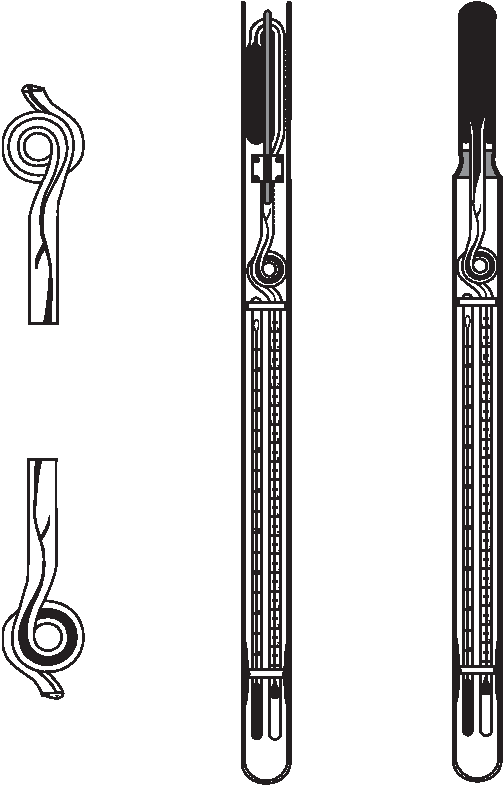
\includegraphics{thermometer}}
%% \footnotesize
%% Figure 6.11 \textbf{Left}: Protected \rule{0mm}{4ex} and unprotected
%% reversing thermometers\index{thermometer!reversing} is set position,
%% before reversal.  \textbf{Right}: The constricted part of the
%% capillary in set and reversed positions. After von Arx (1962: 259).
%% \label{fig:thermometer}
%% \vspace{-3ex}
%% \end{figure}

Один из наиболее важных типов термометров~--- это опрокидывающийся
термометр, который устанавливается на батометрах, описанных в следующем
разделе. В капилляре этого термометра имеется сужение, вызывающее отрыв
столбика ртути при переворачивании термометра вверх дном. Термометр
погружается в океан в нормальном положении и выдерживается до принятия
ним температуры окружающей воды. Ртуть расширяется, и её количество в
капилляре становится пропорциональным температуре. Затем термометр
переворачивается; столбик ртути отрывается и остаётся в капилляре, а
батометр с термометром возвращают на поверхность. Показания с
опрокидывающегося термометра снимаются на палубе вместе с показаниями
обычного термометра, с помощью которого определяют температуру при
снятии показаний. Вместе эти данные позволяют определить температуру 
на глубине в момент переворачивания термометра.
%
% One very important mercury thermometer is the reversing
% thermometer\index{thermometer!reversing} (figure 6.11) carried on
% Nansen bottles, which are described in the next section. It is a
% thermometer that has a constriction in the mercury capillary that
% causes the thread of mercury to break at a precisely determined point
% when the thermometer is turned upside down. The thermometer is lowered
% deep into the ocean in the normal position, and it is allowed to come
% to equilibrium with the water. Mercury expands into the capillary, and
% the amount of mercury in the capillary is proportional to
% temperature. The thermometer is then flipped upside down, the thread
% of mercury breaks trapping the mercury in the capillary, and the
% thermometer is brought back. The mercury in the capillary of the
% reversed thermometer is read on deck along with the temperature of a
% normal thermometer, which gives the temperature at which the reversed
% thermometer is read. The two readings give the temperature of the
% water at the depth where the thermometer was reversed.


Опрокидывающийся термометр находится внутри стеклянной трубки, которая
защищает его от воздействия давления воды, так как оно может
выжать дополнительный объём ртути в капилляр. Если термометр не защищён,
мнимая температура снятая на палубе, будет пропорциональна температуре
и давлению на глубине, где термометр был перевёрнут. Пара из
защищённого и незащищённого термометров даёт температуру и давление на
этой глубине.
%
% The reversing thermometer\index{thermometer!reversing} is carried
% inside a glass tube which protects the thermometer from the ocean's
% pressure because high pressure can squeeze additional mercury into the
% capillary. If the thermometer is unprotected, the apparent temperature
% read on deck is proportional to temperature and pressure at the depth
% where the thermometer was flipped. A pair of protected and unprotected
% thermometers gives temperature and pressure of the water at the depth
% the thermometer was reversed.

Опрокидывающиеся термометры, установленные попарно на батометрах, были 
в период~1900--1970~гг.\ основным источником информации о температуре 
как функции давления. 
%
% Pairs of reversing thermometers\index{thermometer!reversing} carried
% on Nansen bottles were the primary source of sub-sea measurements of
% temperature as a function of pressure from around 1900 to 1970.

%% Рисунок 6.13 Левый: Закрытый и открытый опрокидывающиеся термометры в
%% положении до опрокидывания. Правый: Суженная часть капилляра в
%% изначальном и перевёрнутом положении (Взято из von Arx, 1962).
\end{paragraph}

\begin{paragraph}{Платиновый термометр сопротивления.} 
% \paragraph{Platinum Resistance Thermometer} 
Это стандартный измеритель температуры. Он используется национальными
метрологическими лаборатории для интерполирования между определёнными
точками практической температурной шкалы. Его основное предназначение~---
калибровка других датчиков температуры.
%
% This is the standard for temperature.  \index{temperature!measurement
% at surface!by platinum resistance thermometers}It is used by national
% standards laboratories to interpolate between defined points on the
% practical temperature scale. It is used primarily to calibrate other
% temperature sensors.
\end{paragraph}

\begin{paragraph}{Термистор.}
% \paragraph{Thermistor} 
Термистор~--- это полупроводник, сопротивление которого
предсказуемо и быстро изменяется с изменением
температуры. Термисторы широко используются в стационарных
(заякоренных) и судовых инструментах. Они обладают
высоким разрешением и точностью~$\pm\degCent{0.001}$ при хорошей
калибровке.
%
% A thermistor is a semiconductor having \index{temperature!measurement
% at surface!by thermistors}\index{thermistor}resistance that varies
% rapidly and predictably with temperature. It has been widely used on
% moored instruments and on instruments deployed from ships since about
% 1970.  It has high resolution and an
% accuracy\index{accuracy!temperature!thermistor} of about
% $\pm$0.001\degrees{C} when carefully calibrated.
\end{paragraph}

\begin{paragraph}{Bucket Temperatures.}
% \paragraph{Bucket temperatures.} 
Температура поверхности моря обычно измеряется с помощью ртутного
термометра, помещённого в ведро, опущенное за борт; его выдерживают на
глубине около метра в течении нескольких минут, а затем поднимают на
борт и снимают показания, пока температура в ведре не успела
измениться. Точность~--- около~$\degCent{0.1}$.
%
% The temperature of surface waters has been
% \index{temperature!measurement at surface!by bucket
% thermometers}routinely measured at sea by putting a mercury
% thermometer into a bucket which is lowered into the water, letting it
% sit at a depth of about a meter for a few minutes until the
% thermometer comes to equilibrium, then bringing it aboard and reading
% the temperature before water in the bucket has time to change
% temperature. The accuracy\index{accuracy!temperature!bucket} is around
% 0.1\degrees{C}.  This is a very common source of direct surface
% temperature measurements.
\end{paragraph}

\begin{paragraph}{Температура забираемой воды.}
% \paragraph{Ship Injection Temperature} 
Температура забортной воды, забираемой в систему охлаждения судовых машин,
регулярно записывается в течение десятилетий. Эти значения темературы называют
инжекторной температурой (?). Ошибки в ходе её измерения обусловлены нагревом
воды от корабельных конструкций перед измерением. Это происходит тогда,
когда датчик температуры находится далеко от точки забора на корпусе судна.
Точность этого метода~--- $0.5$--$\degCent{1}$.
%
% The temperature of the water drawn into \index{temperature!measurement
% at surface!from ship injection temperatures}the ship to cool the
% engines has been recorded routinely for decades. These recorded values
% of temperature are called injection temperatures. Errors are due to
% ship's structure warming water before it is recorded. This happens
% when the temperature recorder is not placed close to the point on the
% hull where water is brought in. 
% Accuracy\index{accuracy!temperature!ship-injection} is 
% 0.5\degrees--1\degrees C.
\end{paragraph}

\begin{paragraph}{Улучшенный радиометр очень высокого разрешения~AVHRR.}
% \paragraph{Advanced Very High Resolution Radiometer} 
Этот инструмент наиболее часто используется для измерения температуры морской
поверхности. Он был установлен на всех полярно-орбитальных метеорологических 
спутниках НУОА, начиная с Tiros-N в 1978~г.
%
% The most commonly \index{temperature!measurement at surface!by
% Advanced Very High Resolution Radiometer (AVHRR)}\index{Advanced Very
% High Resolution Radiometer (AVHRR)|textbf}used instrument to measure
% sea-surface temperature from space is the Advanced Very High
% Resolution Radiometer \textsc{avhrr}. The instrument has been carried
% on all polar-orbiting meteorological satellites operated by
% \textsc{noaa} since Tiros-N was launched in 1978.

Инструмент был изначально разработан для измерения температуры
облаков, а следовательно, их высоты. Однако, его точность и прецизионность
оказались достаточными, чтобы вскоре он был задействован для измерения
temperature patterns морской поверхности в глобальном и региональном масштабе.
%
% The instrument was originally designed to measure cloud temperatures
% and hence cloud height. The instrument had, however, sufficient
% accuracy\index{accuracy!AVHRR temperature} and precision that it was
% soon used to measure regional and global temperature patterns at the
% sea surface.

AVHRR представляет собой радиометр, преобразующий инфракрасное излучение
в электрические сигналы. В его конструкцию входит зеркало, которое
сканирует полосу земной поверхности вдоль подспутниковой трассы
и отражает излучение этой полосы в телескоп, фокусирующий его 
на детекторах, чувствительных к различным длинам волн. Детекторы, в свою 
очередь, переводят излучение на этих частотах в электрический сигнал, который
оцифровывается при помощи электронной схемы, где затем и хранится.
Полоса сканирования в ширину составляет~$2700\km$; подспутниковая трасса 
проходит в её центре. Все наблюдения вдоль полосы сканирования состоят 
из пикселов диаметром примерно~$1\km$ у центра полосы; по мере удаления 
от него диаметр увеличивается.
%
% The instrument is a radiometer that converts infrared radiation into
% an electrical voltage. It includes a mirror that scans from side to
% side across the sub-satellite track and reflects radiance from the
% ground into a telescope, a telescope that focuses the radiance on
% detectors, detectors sensitive to different wavelengths that convert
% the radiance at those wavelengths into electrical signals, and
% electronic circuitry to digitize and store the radiance values. The
% instruments observes a 2700-km wide swath centered on the
% sub-satellite track. Each observation along the scan is from a pixel
% that is roughly one kilometer in diameter near the center of the scan
% and that increases in size with distance from the sub-satellite track.

Радиометры измеряют инфракрасную радиацию, излучаемую поверхностью в
пяти диапазонах: трёх инфракрасных ($3.55$--$3.99\mum$, $10.3$--$11.3\mum$,
и~$11.5$--$12.5\mum$), одном ближней инфракрасной части спектра 
($0.725$--$1.10\mum$) и одном видимом ($0.55$--$0.90\mum$). Все инфракрасные
диапазоны включают в себя излучение, испускаемое как морской поверхностью, так
и водяными парами, содержащимися в воздухе на всём пути от спутника до Земли. 
Диапазон~$3.7\mum$ наименее чувствителен к водяному пару и другим помехам, 
но он доступен для наблюдений только ночью, так как днём его заполняет 
излучение Солнца. Два наиболее длинноволновых диапазона, $10.8\mum$ 
и~$12.0\mum$, используются для наблюдения за температурой морской поверхности 
и водяными парами при дневном свете.
%
% The radiometers measures infrared radiation emitted from the surface
% in five wavelength bands: three infrared bands: 3.55--3.99 $\mu$m,
% 10.3--11.3 $\mu$m, and 11.5--12.5 $\mu$m; a near-infrared band at
% 0.725--1.10 $\mu$m; and a visible-light band at 0.55--0.90 $\mu$m. All
% infrared bands include radiation emitted from the sea and from water
% vapor in the air along the path from the satellite to the ground.  The
% 3.7 $\mu$m band is least sensitive to water vapor and other errors,
% but it works only at night because sunlight has radiance in this
% band. The two longest wavelength bands at 10.8 $\mu$m and 12.0 $\mu$m
% are used to observe sea-surface temperature and water vapor along the
% path in daylight.

Данные с разрешением~$1\km$ передаются непосредственно на наземную
станцию, в поле зрения которой находится пролетающий спутник. Это~--- режим
покрытия ограниченного района. Данные также осредняются для получения 
наблюдений с размерами пикселей~$4\times 4\km$. Эти данные сохраняются 
бортовой аппаратурой и в дальнейшем передаются на принимающие станции НУОА. 
Такой режим называется режимом глобального покрытия.
%
% Data with 1-km resolution are transmitted directly to ground stations
% that view the satellite as it passes the station. This is the Local
% Area Coverage mode. Data are also averaged to produce observations
% from 4 $\times$ 4 km pixels. These data are stored by the satellite
% and later transmitted to \textsc{noaa} receiving stations. This is the
% Global Area Coverage mode.

Полоса сканирования достаточно широка для того, чтобы спутник
обследовал все районы Земли дважды в день, приблизительно в 9:00 и
21:00 по местному времени. Районы в высоких широтах могут быть
обследованы более восьми раз за день.
%
% The swath width is sufficiently wide that the satellite views the
% entire earth twice per day, at approximately 09:00 AM and 9:00 PM
% local time. Areas at high latitudes may be observed as often as eight
% or more times per day.

%% \begin{figure}[b!]
%% \vspace{-2ex}
%% \makebox [121mm][c]{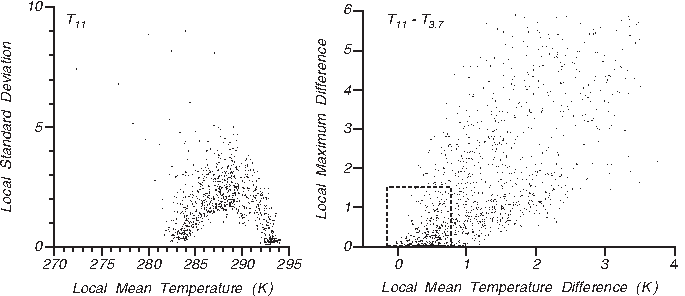
\includegraphics{cloudalgo}}
%% \footnotesize
%% Figure 6.12 The influence \rule{0pt}{4ex}of clouds on infrared
%% observations.  \textbf{Left:} The standard deviation of the radiance
%% from small, partly cloudy areas each containing 64 pixels. The feet of
%% the arch-like distribution of points are the sea-surface and cloud-top
%% temperatures. After Coakley and Bretherton (1982). \textbf{Right:} The
%% maximum difference between local values of $T_{11} - T_{3.7}$ and the
%% local mean values of the same quantity. Values inside the dashed box
%% indicate cloud-free pixels. $T_{11}$ and $T_{3.7}$ are the apparent
%% temperatures at 11.0 and 3.7 $\mu$m (data from K. Kelly). After
%% Stewart (1985: 137).
%% \label{fig:cloudalgo}
%% %\vspace{-3ex}
%% \end{figure}

Причины ошибок, возникающих при измерении температуры поверхности океана. 
%
% The most important errors are due to:\index{temperature!measurement at
% surface!errors in|(}
%
\begin{enumerate}
\item
Unresolved или необнаруженные облака: большие толстые
облака хорошо видны на изображениях температуры воды. Тонкие облака,
такие как низкие слоистые и высокие перистые, вызывают гораздо меньшие 
погрешности, которые трудно или почти невозможно обнаружить. Облака диаметром
менее~$1\km$, такие как пассатные кучевые, также трудно обнаружить. Для
обнаружения небольших облаков были разработаны особые методы (рис.~6.12).
%
% Unresolved or undetected clouds: Large, thick clouds are obvious in
% the images of water temperature Thin clouds such as low stratus and
% high cirrus produce much small errors that are difficult or almost
% impossible to detect. Clouds smaller in diameter than 1 km, such as
% trade-wind cumuli, are also difficult to detect. Special techniques
% have been developed for detecting small clouds (figure 6.12).

\item
Водяной пар, который абсорбирует часть энергии, излучаемой поверхностью
моря: водяной пар уменьшает получаемую(?) температуру морской
поверхности. Его влияние в диапазонах~$10.8\mum$ и~$12.0\mum$ различается,
что позволяет использовать отличия между сигналами для уменьшения погрешности.
%
% Water vapor, which absorbs part of the energy radiated from the sea
% surface: Water vapor reduces the apparent temperature of the sea
% surface. The influence is different in the 10.8 $\mu$m and 12.0 $\mu$m
% channels, allowing the difference in the two signals to be used to
% reduce the error.  

\item
Аэрозоли, поглощающие инфракрасную радиацию. Они излучают при
температурах, встречающихся в верхней атмосфере. Стратосферные аэрозоли,
порождённые извержениями вулканов, могут понизить наблюдаемые
температуры на несколько градусов Цельсия. Частички пыли от пылевых
бурь в Сахаре, распространяемые над Атлантикой, также могут приводить к
погрешностям.
%
% Aerosols, which absorb infrared radiation. They radiate at
% temperatures found high in the atmosphere. Stratospheric aerosols
% generated by volcanic eruptions can lower the observed temperatures by
% up to a few degrees Celsius. Dust particles carried over the Atlantic
% from Saharan dust storms can also cause errors.


%% \item
%% Инструментальные помехи стремятся уменьшить, ограничивая
%% температурное разрешение на изображениях локальных районов.

\item
Ошибки температуры скин-слоя. Инфракрасная радиация, фиксируемая
инструментом, приходит из слоя на морской поверхности толщиной в
несколько микрометров. Температура в этом слое не такая же, как в метре
под поверхностью. При слабом ветре она может отличаться на несколько
градусов (Emery and Schussel, 1989). Этот источник погрешности может быть
существенно ослаблен, если данные AVHRR используются для интерполяции между
точками судовых измерений поверхностной температуры.
%
% Skin temperature errors. The infrared radiation seen by the instrument
% comes from a layer at the sea surface that is only a few micrometers
% thick. The temperature in this layer is not quite the same as
% temperature a meter below the sea surface. They can differ by several
% degrees when winds are light (Emery and Schussel,
% 1989).\index{temperature!measurement at surface!errors in|)} This
% error is greatly reduced when \textsc{avhrr} \index{Advanced Very High
% Resolution Radiometer (AVHRR)}data are used to interpolate between
% ship measurements of surface temperature.
\end{enumerate}

Карты температуры, созданные на основе измерений в режиме покрытия 
ограниченного района при отсутствии облаков, показывает изменчивость 
температуры с точностью~$\degCent{0.1}$. Эти карты используются для 
изучения локальных явлений, включая структуры, образованные местными 
течениями. Рис.~10.16 демонстрирует такие структуры у побережья Калифорнии.
%
% Maps of temperature processed from Local Area Coverage of cloud-free
% regions show variations of temperature with a precision of
% 0.1\degrees{C}. These maps are useful for observing local phenomena
% including patterns produced by local currents. Figure 10.16 shows such
% patterns off the California coast.

Глобальные карты составляются Океанографической службой ВМС США, которая
%% toindex: U.S. Naval Oceanographic Office
получает глобальные данные с AVHRR напрямую из Национальной службы 
по информации, данным и спутникам для исследования окружающей среды (НЕСДИС)
%% toindex: National Environmental Satellite Data and Information Service 
ежедневно в режиме, близком к реальному времени. Эти данные тщательно
обрабатываются для устранения влияния облаков, водяного пара,
аэрозолей, и других источников ошибок. Затем они используются для
создания карт между~$\pm\degrees{70}$ с точностью~$\pm\degCent{0.6}$
(May et al 1998). Карты температуры поверхности океана пересылаются ВМФ США
и в Национальные центры по прогнозированию окружающей среды НУОА.
Кроме того, служба ежедневно составляет 100-км
глобальные и 14-км региональные карты температуры.
%% что имеется в виду? шаг сетки?
%
% Global maps are made by the U.S. Naval Oceanographic Office, which
% receives the global \textsc{avhrr} \index{Advanced Very High
% Resolution Radiometer (AVHRR)}data directly from \textsc{noaa}'s
% National Environmental Satellite, Data and Information Service in
% near-real time each day. The data are carefully processed to remove
% the influence of clouds, water vapor, aerosols, and other sources of
% error. Data are then used to produce global maps between $\pm
% 70$\degrees\ with an accuracy\index{accuracy!AVHRR temperature!maps}
% of $\pm 0.6$\degrees{C} (May et al 1998). The maps of sea-surface
% temperature are sent to the U.S. Navy and to \textsc{noaa}'s National
% Centers for Environmental Prediction. In addition, the office produces
% daily 100-km global and 14-km regional maps of temperature.

%% Рисунок 6.14 Влияние облаков на инфракрасные наблюдения. Слева:
%% Стандартное отклонение излучения для небольших частично облачных
%% районов, содержащих по 64 пиксела каждый. Основанием для наиболее
%% вероятного распределения точек являются температура поверхности моря и
%% верхних облаков. (Следуя Coakley and Bretherton (1982). Справа:
%% Максимальные различия между локальными значениями T11- T3.7 и
%% локальными средними значениями того же параметра. Пунктирный квадрат
%% ограничевает значения пикселов свободных от влияния облаков. T11 и
%% T3.7 мнимые температуры на 11.0 и 3.7 микрометрах (данные
%% K. Kelly). Взято из Stewart (1985).
\end{paragraph}

\begin{paragraph}{Глобальные карты температуры поверхности океана.}
% \paragraph{Global Maps of Sea-Surface Temperature}
Глобальные ежемесячные карты поверхностной температуры создаются
Национальными центрами по прогнозированию окружающей среды
с использованием метода оптимальной интерполяции Рейнольдса Reynolds et al (2002). 
При помощи этого метода корабельные и буйковые наблюдения поверхностной 
температуры объединяются с данными AVHRR, обработанными Океанографической 
службой ВМС с пространственным разрешением~$\degrees{1}$ и временным~---
один месяц. Essentially, AVHRR data are interpolated between buoy 
and ship reports using previous information about the temperature field.
Итоговая точность лежит в диапазоне от примерно~$\pm\degCent{0.3}$ в тропиках
до~$\pm\degCent{0.5}$ в районе западных пограничных течений в северном
полушарии, где температурные градиенты велики. Доступны карты с ноября 
1981~г.\ по настоящее время. Рис.~6.2--6.4 сделаны на основе данных,
обработанных НУОА по методу Рейнольдса. Другие комплекты данных были
получены НУОА/НАСА в рамках программы Pathfinder (Kilpatrick, Podesta, and Evans, 2001).
%
% Global, monthly maps of \index{temperature!global maps of}surface
% temperature are produced by the National Centers for Environmental
% Prediction using Reynolds et al (2002) optimal-interpolation
% method. The technique blends ship and buoy measurements of sea-surface
% temperature with \textsc{avhrr} \index{Advanced Very High Resolution
% Radiometer (AVHRR)}data processed by the Naval Oceanographic Office in
% 1\degrees\ areas for a month. Essentially, \textsc{avhrr} data are
% interpolated between buoy and ship reports using previous information
% about the temperature field. Overall
% accuracy\index{accuracy!temperature!sea-surface maps} ranges from
% approximately $\pm 0.3$\degrees\ C in the tropics to $\pm
% 0.5$\degrees\ C near western boundary currents in the northern
% hemisphere where temperature gradients are large.  Maps are available
% from November 1981. Figures 6.2--6.4 were made by \textsc{noaa} using
% Reynolds' technique. Other data sets have been produced by the
% \textsc{noaa/nasa} Pathfinder program (Kilpatrick, Podesta, and Evans,
% 2001).

Карты средних температур также составлялись на основе данных 
ИКОАДС (Smith and Reynolds, 2004). Вследствие их неравномерного 
пространственного и временного распределения, погрешность также изменяется
во времени и пространстве. Смит и Рейнольдс Smith and Reynolds (2004) 
оценили погрешность глобальной средней температуры и обнаружили, что
при доверительной вероятности~95\% доверительные границы погрешности
near-global average равны~$\degCent{0.48}$ или более в XIX~веке, 
около~$\degCent{0.28}$ в первой половине XX~века и~$\degCent{0.18}$ 
или менее после 1950~г. Аномалии поверхностной температуры рассчитывались 
с использованием данных ИКОАДС о средних поверхностных температурах 
за период 1854--1997~гг., дополненных спутниковыми данными с 1981~г.
%
% Maps of mean temperature have also been made from \textsc{icoads}
% \index{ICOADS (international comprehensive ocean-atmosphere data
% set)}data (Smith and Reynolds, 2004). Because the data are poorly
% distributed in time and space, errors also vary in time and
% space. Smith and Reynolds (2004) estimated the error in the global
% mean temperature and found the 95\% confidence uncertainty for the
% near-global average is 0.48\degrees\ C or more in the nineteenth
% century, near 0.28\degrees\ C for the first half of the twentieth
% century, and 0.18\degrees\ C or less after
% 1950. Anomalies\index{anomalies!sea-surface temperature} of
% sea-surface temperature were calculated using mean sea-surface
% temperature from the period 1854--1997 using
% \textsc{icoads}\index{ICOADS (international comprehensive
% ocean-atmosphere data set)} supplemented with satellite data since
% 1981.
\end{paragraph}
\end{section}

\begin{section}{Измерения электропроводности и солёности}
% \section{Measurement of Conductivity or Salinity}
%% Измерения электропроводности могут быть произведены с использованием
%% электродов, но электроды имеют тенденцию отклоняться от стандартного
%% напряжения в результате электрохимических процессов. Помните, два
%% разных металла покружённых в электропроводящий раствор, образуют
%% батарею.
%% 
%% Измерения обычно проводятся с использованием индукции. Морская вода
%% формирует одну часть трансформатора, и ток индуцируемый в катушке
%% трансформатора зависит от электропроводности морской воды (Рисунок
%% 6,15). Эта техника устраняет электрохимические отклонения от
%% стандартного напряжения. Лучшие измерения солёности по
%% электропроводности дают солёность с точностью~$0.005\psu$
%%
Для измерения электропроводности в морскую воду помещают платиновые электроды,
после чего измеряют силу тока, протекающего между ними при заданном напряжении.
%%
%% current --- досл. "ток" или "сила тока"?
%% http://en.wikipedia.org/wiki/Ampere
%% The ampere (symbol: A) is the SI unit of electric current and is one 
%% of the seven SI base units
%%
Эта сила зависит от электропроводности, напряжения и объема воды, заключенного 
между электродами. Если поместить электроды в изолирующую стеклянную трубку,
объем воды будет точно известен, а сила тока~--- независима от других объектов
вблизи conductivity cell (рис.~6.13). Наилучшая точность, достигнутая в ходе
измерения солёности по электропроводности, составляет~$\pm 0.005$.
% 
% \index{conductivity!measurement of}Conductivity is measured by placing
% platinum electrodes in seawater and measuring the current that flows
% when there is a known voltage between the electrodes. The current
% depends on conductivity, voltage, and volume of sea water in the path
% between electrodes. If the electrodes are in a tube of non-conducting
% glass, the volume of water is accurately known, and the current is
% independent of other objects near the conductivity cell (figure
% 6.13). The best measurements of salinity from conductivity give
% salinity with an accuracy\index{accuracy!salinity} of $\pm$0.005.

До того, как измерения электропроводности вошли в повседневную практику,
для определения солёности применяли титрование пробы воды
солями серебра. Максимальная точность этого метода равна $\pm 0.02$.
%
% Before conductivity measurements were widely used, salinity
% \index{salinity!measurement of}was measured using chemical titration
% of the water sample with silver salts. The best measurements of
% salinity from titration give salinity with an
% accuracy\index{accuracy!salinity!from titration} of $\pm$0.02.

%% \begin{figure}[t!]
%% %\vspace{-2ex}
%% \makebox[120mm] [c] {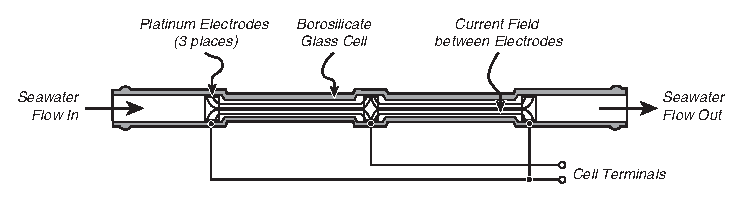
\includegraphics{conductivity}}
%% \footnotesize
%% Figure 6.13 A conductivity \rule{0pt}{4ex}cell. Current flows through
%% the seawater between platinum electrodes in a cylinder of borosilicate
%% glass 191 mm long with an inside diameter between the electrodes of 4
%% mm. The electric field lines (solid lines) are confined to the
%% interior of the cell in this design making the measured conductivity
%% (and instrument calibration) independent of objects near the
%% cell. This is the cell used to measure conductivity and salinity shown
%% in figure 6.15. From Sea-Bird Electronics.
%% \label{fig:conductivity}
%% \vspace{-3ex}
%% \end{figure}

Калибровка инструментов, измеряющих солёность, может быть проведена на
стандартной морской воде. Долгосрочные исследования точности таких измерений
ведутся на основе результатов исследования солёности глубинных водных масс,
которая отличается высокой стабильностью. Так, например, 
Саундерс (Saunders 1986) заметил строгую взаимосвязь температуры и солёности 
большого объема воды, расположенного в глубокой котловине на северо-востоке 
Атлантического океана под Средиземноморским противотечением. Он воспользовался
согласованностью измерений температуры и солёности, произведенных на большом
количестве гидрографических станций в этом районе для того, чтобы оценить 
точность измерения температуры, солёности и содержания кислорода. Был сделан 
вывод, что наиболее тщательные измерения, произведенные после 1970~г., имеют 
точность~$0.005$ для солёности и~$\degCent{0.005}$ для температуры. 
Самым большим источником ошибок в случае солёности была ошибка при 
determination стандартной воды, используемой для калибровки.
%
% Individual salinity measurements \index{salinity!measurement of}are
% calibrated using standard seawater. Long-term studies of
% accuracy\index{accuracy!salinity} use data from measurements of deep
% water masses of known, stable, salinity. For example, Saunders (1986)
% noted that temperature is very accurately related to salinity for a
% large volume of water contained in the deep basin of the northwest
% Atlantic under the Mediterranean outflow. He used the consistency of
% measurements of temperature and salinity made at many hydrographic
% stations\index{hydrographic stations!used for salinity} in the area to
% estimate the accuracy\index{accuracy!salinity} of temperature,
% salinity and oxygen measurements. He concluded that the most careful
% measurements made since 1970 have an accuracy of 0.005 for salinity
% and 0.005\degrees{C} for temperature. The largest source of salinity
% error was the error in determination of the standard water used for
% calibrating the salinity measurements.

%% \begin{figure}[t!]
%% %\vspace{-3ex}
%% 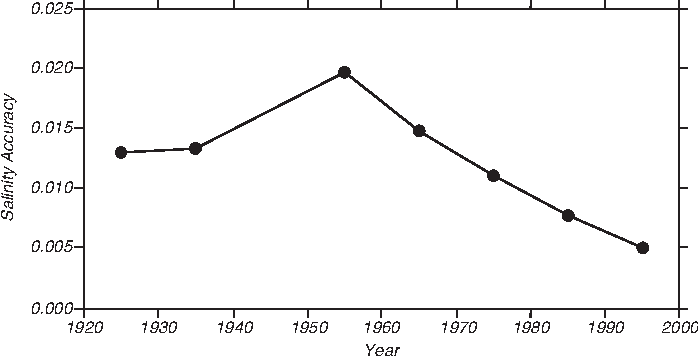
\includegraphics{salinityaccuracy}
%% \footnotesize
%% Figure 6.14. Standard deviation \rule{0mm}{3ex}of salinity
%% measurements below 1500 m in the south Atlantic. Each point is the
%% average for the decade centered on the point. The value for 1995 is an
%% estimate of the accuracy\index{accuracy!salinity} of recent
%% measurements. From Gouretski and Jancke (1995).
%% \label{fig:salinityaccuracy}
%% \vspace{-4ex}
%% \end{figure}
%% 
%% \begin{figure}[b!]
%% \vspace{-4ex}
%% \makebox [120mm][c]{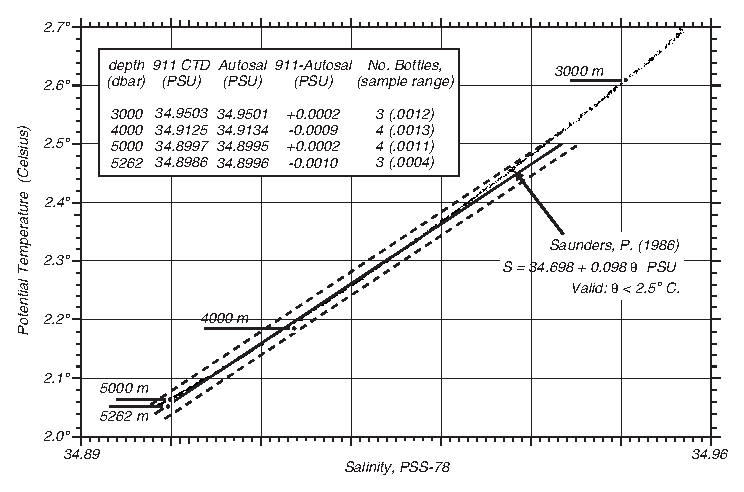
\includegraphics{911data}}
%% \footnotesize
%% Figure 6.15. Results from \rule{0pt}{3ex}a test of the Sea-Bird
%% Electronics 911 Plus CTD\index{CTD} in the North Atlantic Deep
%% Water\index{North Atlantic Deep Water} in 1992. Data were collected at
%% 43.17\degrees\ N and 14.08\degrees\ W from the R/V Poseidon. From
%% Sea-Bird Electronics (1992).
%% \label{fig:911data}
%% %\vspace{-3ex}
%% \end{figure}

Gouretski и Jancke (Gouretski and Jancke 1995) оценили точность
измерений солёности как функцию времени. Используя
высококачественные измерения с $16\,000$~гидрографических станций в
южной Атлантике с~1912 по~1991~гг., они дали оценку точности, представив
солёность как функцию температуры на основе всех данных, полученных на 
глубинах свыше~$1500\m$ в двенадцати областях за каждое десятилетие в период
с~1920 по~1990~гг. График точности как функции времени за период с 1920~г.\ %
показал последовательное улучшение точности, начиная с 1950~г.\ (рис.~6.14). 
Современные измерения солёности наиболее точны. Стандартное отклонение 
современных данных по солёности, собранных во всех южных регионах 
Атлантического океана с~1970 по~1993~гг.\ и исправленных согласно предложенной
Gouretski и Jancke (Gouretski and Jancke 1995) методике, составляло~$0.0033$.
Более современные инструменты, такие как 
\emph{Sea-Bird Electronics Model 911 Plus}, обладают точностью свыше~$0.005$ 
без поправок. Тщательное сравнение солёности, измеренной в 
точке~\latlonmin{43}{10}{N} \latlonmin{14}{4.5}{W} при помощи
\emph{Sea-Bird Electronics Model 911 Plus} с историческими данными, собранными
Саундерсом (Saunders 1986) даёт точность в~$0.002$ (рис.~6.15).
%
% Gouretski and Jancke (1995) estimated
% accuracy\index{accuracy!salinity}\index{salinity!accuracy of}of
% salinity measurements as a function of time. Using high quality
% measurements from 16,000 hydrographic stations\index{hydrographic
% stations!used for salinity} in the south Atlantic from 1912 to 1991,
% they estimated accuracy by plotting salinity as a function of
% temperature using all data collected below 1500 m in twelve regions
% for each decade from 1920 to 1990. A plot of accuracy as a function of
% time since 1920 shows consistent improvement in accuracy since 1950
% (figure 6.14). Recent measurements of salinity are the most
% accurate. The standard deviation of salinity data collected from all
% areas in the south Atlantic from 1970 to 1993 adjusted as described by
% Gouretski and Jancke (1995) was 0.0033. Recent instruments such as the
% Sea-Bird Electronics Model 911 Plus have an
% accuracy\index{accuracy!salinity} of better than 0.005 without
% adjustments. A comparison of salinity measured at 43\degrees\ 10\'{}N,
% 14\degrees\ 4.5\'{}W by the 911 Plus with historic data collected by
% Saunders (1986) gives an accuracy of 0.002 (figure 6.15).

%% Figure 6.13 A conductivity cell. Current flows through the seawater
%% between platinum electrodes in a cylinder of borosilicate glass 191mm
%% long with an inside diameter between the electrodes of 4mm. The
%% electric field lines (solid lines) are confined to the interior of the
%% cell in this design making the measured conductivity (and instrument
%% calibration) independent of objects near the cell. This is the cell
%% used to measure conductivity and salinity shown in Figure 6.15. From
%% Sea-Bird Electronics.
%% 
%% Рисунок 6.16. Стандартное отклонение измерений солёности на глубине
%% 1500 м в Южной Атлантике с 1920 по 1993 год. Каждая точка~--- среднее
%% данных собранных за десятилелие. Значение для 1995 года представляет
%% собой точность современных измерений. Взято из Таблицы 1 в Gouretski
%% and Jancke (1995).
%% 
%% Рисунок 6.17. Результаты тестирования Sea-Bird Electronics 911 Plus
%% CTD выполненного в Северо Атлантических глубинных водах в 1992
%% году. (Взято из Sea-Bird Electronics, 1992).
\end{section}

\begin{section}{Измерения давления}
% \section{Measurement of Pressure}
Давление измеряется разными типами инструментов. Единицей давления в
системе СИ является паскаль, но океанографы обычно используют децибары:
\begin{equation}
1\dBar = 10^4\Pa,
\end{equation}
поскольку давление в децибарах почти точно соответствует глубине в
метрах. Таким образом, $1000\dBar$~--- это давление на глубине 
около~$1000\m$.
%
% \index{pressure!measurement of}Pressure is routinely measured by many
% different types of instruments. The SI unit of pressure is the pascal
% (Pa), but oceanographers normally report pressure in decibars (dbar),
% where:
% \begin{equation}
% 1 \text{ dbar} = 10^4 \text{ Pa}
% \end{equation}
% because the pressure in decibars is almost exactly equal to the depth
% in meters.  Thus 1000 dbar is the pressure at a depth of about 1000 m.


\begin{paragraph}{Датчик деформации или тензодатчик.}
% \paragraph{Strain Gage}
Это наиболее простой, дешевый и популярный инструмент. 
Его точность~--- около~$\pm 1\%$.
%
% \index{pressure!measurement of!strain gage}
% This is the simplest and cheapest instrument, \index{strain gage}and
% it is widely used. Accuracy\index{accuracy!pressure} is about
% $\pm$1\%.
\end{paragraph}

\begin{paragraph}{Вибратрон.}
% \paragraph{Vibratron}
Гораздо более точные измерения давления могут быть выполнены путем
измерения собственной частоты вибрирующей вольфрамовой проволоки,
натянутой в магнитном поле между мембранами, закрывающими концы
цилиндра. Давление изгибает мембраны, которые меняют натяжение проволоки, а
следовательно, и частоту вибрации. Частоту можно измерить по изменению 
электрического напряжения, которое индуцируется в вибрирующей в магнитном поле 
проволоке. Точность~--- около~$\pm 0.1\%$, а при контроле температуры ещё выше. 
Прецизионность в 100--1000~раз выше, чем точность. Инструмент используется 
для обнаружения малых изменений давления на больших глубинах. 
Снодграсс Snodgrass (1968) получил прецизионность в~$\pm 0.8\mm$ на 
глубине~$3\km$.
%
% Much more accurate measurements of pressure can be
% \index{pressure!measurement of!vibratron}\index{vibratron}made by
% measuring the natural frequency of a vibrating tungsten wire stretched
% in a magnetic field between diaphragms closing the ends of a
% cylinder. Pressure distorts the diaphragm, which changes the tension
% on the wire and its frequency. The frequency can be measured from the
% changing voltage induced as the wire vibrates in the magnetic field.
% Accuracy\index{accuracy!pressure} is about $\pm$0.1\%, or better when
% temperature controlled. Precision is 100--1000 times better than
% accuracy. The instrument is used to detect small changes in pressure
% at great depths. Snodgrass (1964) obtained a precision equivalent to a
% change in depth of $\pm$0.8 mm at a depth of 3 km.
\end{paragraph}

\begin{paragraph}{Кварцевый кристалл.}
% \paragraph{Quartz crystal}
Очень точные измерения давления можно также произвести, измерив
собственную частоту кристалла кварца cut for minimum temperature dependence. 
Наилучшая точность достигается тогда, когда температура 
кристалла остаётся постоянной. Точность составляет~$\pm 0.015\%$, а
разрешение~--- $0.001\%$ (от значения величины).
%
% Very accurate measurements of pressure can also
% \index{pressure!measurement of!quartz crystal}be made by measuring the
% natural frequency of a quartz crystal cut for minimum temperature
% dependence. The best accuracy\index{accuracy!pressure} is obtained
% when the temperature of the crystal is held constant. The accuracy is
% $\pm$0.015\%, and precision is $\pm$0.001\% of full-scale values.
\end{paragraph}

\begin{paragraph}{Кварцевый манометр Бурдона.}
% \paragraph{Quartz Bourdon Gage}
Этот прибор имеет точность и стабильность, сравнимую с кварцевыми кристаллами. 
Он также используется для долговременных измерений давления в глубине
моря.
%
% has accuracy\index{accuracy!pressure} and stability comparable to
% \index{pressure!measurement of!quartz bourdon gage}quartz crystals. It
% too is used for long-term measurements of pressure in the deep sea.
\end{paragraph}
\end{section}


\begin{section}{Измерение зависимости температуры и солёности от глубины}
% \section[Temperature and Salinity With Depth]{Measurement of Temperature and
% Salinity with Depth} 
Температура, солёность и давление измеряются как функция глубины с
помощью различных инструментов и методов, а плотность рассчитывается по
результатам этих измерений.
%
% \index{temperature!measurement with depth}\index{salinity!measurement
% with depth} Temperature, salinity, and pressure are measured as a
% function of depth using various instruments or techniques, and density
% is calculated from the measurements.

\begin{paragraph}{Батитермограф.}
% \paragraph{Bathythermograph (BT)} 
Это механическое устройство, которое показывает профиль температуры 
в зависимости от глубины на закопченном куске стекла. Оно широко
использовалось для картирования термической структуры поверхностных вод, 
включая перемешанный слой, вплоть до замены отрывными батитермографами 
в 1970-х.
%
% was a mechanical device that measured \index{temperature!measurement
% with depth!by bathythermograph (BT)} \index{bathythermograph
% (BT)}temperature vs depth on a smoked glass slide. The device was
% widely used to map the thermal structure of the upper ocean, including
% the depth of the mixed layer\index{mixed layer!measured by
% bathythermograph} before being replaced by the expendable
% bathythermograph in the 1970s.
\end{paragraph}

\begin{paragraph}{Отрывной батитермограф.} 
% \paragraph{Expendable Bathythermograph (XBT)}
Представляет собой электрический прибор, измеряющий изменение температуры 
с глубиной при помощи термистора, установленного на свободно падающем 
обтекаемом грузе. Термистор соединён с омметром на корабле тонкой медной 
проволокой, которая разматывается с тонущего груза и с движущегося корабля. 
В настоящее время отрывной батитермограф, также известный как XBT%
\remark{Англ. expendable bathythermograph}, считается наиболее распространённым
инструментом для измерений вертикальной термической структуры верхнего
океана. Ежегодно используется приблизительно $65\,000$~таких приборов.
%
% is an electronic device that \index{temperature!measurement with
% depth!by expendable bathythermograph (XBT)}\index{bathythermograph
% (BT)!expendable (XBT)}measures temperature vs depth using a thermistor
% on a free-falling streamlined weight. The thermistor is connected to
% an ohm-meter on the ship by a thin copper wire that is spooled out
% from the sinking weight and from the moving ship. The \textsc{xbt} is
% now the most widely used instrument for measuring the thermal
% structure of the upper ocean. Approximately 65,000 are used each year.

%% \begin{figure}[t!]
%% 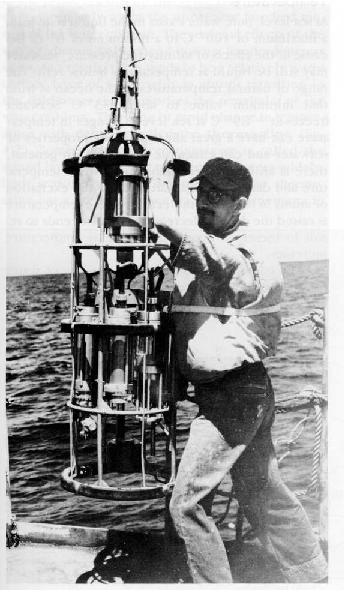
\includegraphics{ctdnansen}
%% \ \ \ \ \ \
%% 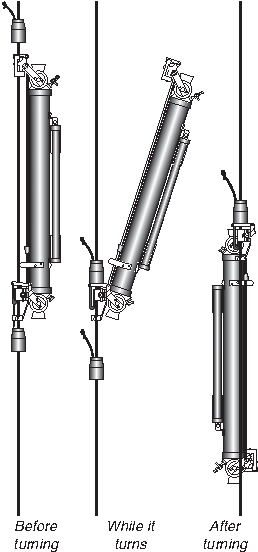
\includegraphics{ctdnansenRight}
%% \ \ \ \ \ \ \\
%% \footnotesize
%% Figure 6.16 \textbf{Left} A CTD \rule{0mm}{4ex}ready to\index{CTD} be
%% lowered over the side of a ship. From Davis (1987). \textbf{Right}
%% Nansen water bottles before (I), during (II), and after (III)
%% reversing. Both instruments are shown at close to the same
%% scale. After Defant (1961: 33).
%% \label{fig:ctdnansen}
%% \vspace{-3ex}
%% \end{figure}

Груз обтекаемой формы погружается в воду с постоянной скоростью. Благодаря
этому, глубина может быть рассчитана по времени погружения с 
точностью~$\pm 2\%$. Точность измерения температуры~$\pm\degCent{0.1}$,
а вертикальное разрешение, как правило, составляет~$65\cm$. В зависимости от
модели устройства, оно достигает глубины от~$200$ до~$1830\m$.
%
% The streamlined weight falls through the water at a constant
% velocity. So depth can be calculated from fall time with an
% accuracy\index{accuracy!depth from XBT} of $\pm$2\%.  Temperature
% accuracy\index{accuracy!temperature!XBT} is $\pm$0.1\degrees{C}.  And,
% vertical resolution is typically 65 cm. Probes reach to depths of 200
% m to 1830 m depending on model.
\end{paragraph}

\begin{paragraph}{Батометр Нансена}
% \paragraph{Nansen Bottles} 
(рис.~6.16). Использовались на кораблях, проводивших гидрографические
станции. \emph{Гидрографические станции}~--- места, где океанографы измеряют
параметры воды от поверхности до некоторой глубины или до дна,
используя инструменты, спускаемые с корабля. Как правило, 20~батометров с
интервалом от нескольких десятков до сотен метров закрепляются на
тросе, погружаемом за борт корабля. Распределение батометров по глубине
выбирается с таким расчётом, чтобы большинство из них находилось в верхних
слоях, где величина изменений температуры по вертикали максимальна.
Защищённые опрокидывающиеся термометры, предназначенные для измерения
температуры, прикрепляются к каждому батометру вместе с незащищённым
опрокидывающимся термометром для измерения глубины. Батометр состоит
из цилиндра с затворами на каждом конце для отбора морской воды на
глубине. Солёность определялась лабораторным анализом этих проб.
%
% (figure 6.16) were deployed from ships stopped at hydrographic
% stations.  \index{temperature!measurement with depth!by reversing
% thermometers} \index{thermometer!reversing!on Nansen
% bottles}\index{Nansen bottles} \textit{Hydrographic stations}
% \index{hydrographic stations|textbf}are places where oceanographers
% measure water properties from the surface to some depth, or to the
% bottom, using instruments lowered from a ship. Usually 20 bottles were
% attached at intervals of a few tens to hundreds of meters to a wire
% lowered over the side of the ship. The distribution with depth was
% selected so that most bottles are in the upper layers of the water
% column where the rate of change of temperature in the vertical is
% greatest. A protected reversing
% thermometer\index{thermometer!reversing} for measuring temperature was
% attached to each bottle along with an unprotected reversing
% thermometer\index{thermometer!reversing} for measuring depth. The
% bottle contains a tube with valves on each end to collect sea water at
% depth. Salinity was determined by laboratory analysis of water sample
% collected at depth.

После того как все батометры были прикреплены к тросу и погружены на
выбранную глубину, вниз по тросу посылается грузик. Этот грузик
заставляет срабатывать механизм, переворачивающий батометр, что, в свою 
очередь, опрокидывает термометры, закрывает клапаны, запирающие воду в
цилиндре, а затем освобождает следующий грузик. Когда все батометры
сработают, их поднимают. Вся станция обычно занимает несколько часов.
%
% After bottles had been attached to the wire and all had been lowered
% to their selected depths, a lead weight was dropped down the wire. The
% weight tripped a mechanism on each bottle, and the bottle flipped
% over, reversing the thermometers\index{thermometer!reversing},
% shutting the valves and trapping water in the tube, and releasing
% another weight. When all bottles had been tripped, the string of
% bottles was recovered. The deployment and retrieval typically took
% several hours.
\end{paragraph}

\begin{paragraph}{CTD.}
% \paragraph{CTD}
Механические инструменты на батометрах Нансена в начале 1960-х были
заменены электронным, получившим название~CTD, которое подчеркивает его
назначение: измерение электропроводности, температуры и глубины%
\remark{Англ.~conductivity, temperature, depth} (рис.~6.16).
Измерения записываются в цифровой форме либо самим инструментом во время 
погружения, либо на корабле. Температура обычно измеряется термистором, 
электропроводность~--- с помощью conductivity cell, а давление~--- 
кварцевым кристаллом. Точность современных инструментов представлена в 
табл.~\ref{tbl:6.2}.
%
% Mechanical instruments on Nansen bottles were replaced
% \index{temperature!measurement with depth!by CTD}\index{CTD}beginning
% in the 1960s by an electronic instrument, called a \textsc{ctd}, that
% measured conductivity, temperature, and depth (figure 6.16). The
% measurements are recorded in digital form either within the instrument
% as it is lowered from a ship or on the ship.  Temperature is usually
% measured by a thermistor. Conductivity is measured by a conductivity
% cell. Pressure is measured by a quartz crystal.  Modern instruments
% have accuracy\index{accuracy!CTD} summarized in table 6.2.

\begin{table}
\caption{Точность Измерений CTD}\label{tbl:6.2}
\begin{tabular}{lll}
\hline
Переменная          & Диапазон       & Наилучшая точность \\
Температура         & $\degCent{42}$ & $\pm \degCent{0.001}$\\
Солёность           & $1$            & $\pm 0.02$ (титрование) \\
                    &                & $\pm 0.005$ (электропроводность)\\
Давление            & $10\,000\dBar$ & $\pm 0.65\dBar$\\
Плотность           & $2\kgpcm$      & $\pm 0.005\kgpcm$\\
Уравнение Состояния &                & $\pm 0.005\kgpcm$ \\
\hline
\end{tabular}
\end{table}
%
% \begin{table}[h!]\small \centering
% \vspace{1ex}
% \begin{tabular*}{95mm}{@{}lr@{}ll@{}}
% \multicolumn{4}{@{}l@{}}{\bfseries Table 6.2 Summary of \rule[-1ex]{0mm}{1ex}Measurement Accuracy}  \\
% \hline
% Variable & Range & & \rule{0ex}{2.5ex}Best Accuracy \\
% \hline
% Temperature & \rule{0ex}{2.5ex}42 &\ \degrees C & $\pm$ 0.001 \degrees C  \\
% Salinity    & 1     &\   & $\pm$ 0.02 by titration          \\
%             &       &       & $\pm$ 0.005 by conductivity      \\
% Pressure    & 10,00 &\ dbar & $\pm$ 0.65 dbar                         \\
% Density     & 2     &\ kg/m$^3$ & $\pm$ 0.005 kg/m$^3$             \\
% Equation of State  &        &   & $\pm$ 0.005 kg/m$^3$             \\ [0.5ex]
% \hline
% \end{tabular*} \\[0.5ex]
% \vspace{-3ex}
% \end{table}

%% Рисунок 6.18 Сверху CTD готов к спуску за борт корабля (Взято из
%% Davis, 1987). Снизу Батометр Нансена до (I), во время (II), и после
%% (III) опрокидывания. Инструменты показаны приблизительно в одном
%% масштабе. (Взято из Dietrich et al. 1980)
\end{paragraph}

\begin{paragraph}{CTD на дрейфующих буях.}
% \paragraph{CTD on Drifters}
Возможно, наиболее общим источником данных о зависимости температуры и 
солёности от глубины в верхних~$2\km$ водной толщи служит множество 
буев-профилографов Argo, которые будут описаны в разд.~\ref{sec:11.8}.
%% в оригинале: ARGOS, НО: http://www.argo.ucsd.edu/ --- Argo 
Эти буи дрейфуют на глубине~$1\km$, погружаются до~$2\km$, а затем всплывают
на поверхность. Они измеряют температуру и солёность в ходе изменения глубины,
используя инструменты, аналогичные применяемым на~CTD. Данные пересылаются
в центры обработки на суше при помощи системы Argos, установленной на 
полярно-орбитальных спутниках НУОА. В 2006~г.\ примерно 2500 буев генерировали
один профиль каждые 10~дней, покрывая большую часть океана. Точность 
получаемых данных составляет $\degCent{0.005}$~для температуры, 
$5\dBar$~для давления и $0.01$~для солёности (Riser et al, 2008).
%
% Perhaps\index{CTD} the most common source of temperature and salinity
% as a function of depth in the upper two kilometers of the ocean is the
% set of profiling \textsc{argo} floats\index{floats!Argo} described in
% \S{11.8}. The floats drift at a depth of 1 km, sink to 2 km, then rise
% to the surface. They profile temperature and salinity while changing
% depth using instruments very similar to those on a \textsc{ctd}. Data
% are sent to shore via the Argos system\index{Argos system} on the
% \textsc{noaa} polar-orbiting satellites. In 2006, nearly 2500 floats
% were producing one profile every 10 days throughout most of the
% ocean. The accuracy of data from the floats is 0.005\degrees C for
% temperature, 5 decibars for pressure, and 0.01 for salinity (Riser et
% al (2008).
\end{paragraph}

\begin{paragraph}{Комплекты данных.}
% \paragraph{Data Sets}
В рамках проекта Marine Environment and Security For European Area
(MERSEA) опубликована коллекция профилей подповерхностной (потенциальной) 
температуры и солёности \emph{Enact/Ensembles (EN3): Quality Controlled in
situ Ocean Temparature and Salinity Profiles database}. По состоянию 
%% http://www.mersea.eu.org/Insitu-Obs/1-Insitu-Data-ENACT.html
на~2008~г. в этот комплект данных входили: около миллиона профилей~XBT, 
$700\,000$~профилей CTD, и~$60\,000$~--- Argo, а также~$1\,100\,000$
батометрических проб высокого качества, собранных на глубинах до~$700\m$ 
(Domingues et al, 2008).
%% не вполне понятно, к чему относится "качество" и глубина --- ко всем
%% данным или только к батометрическим исследованиям?
%
% \paragraph{Data Sets}
% Data are in the Marine Environment and Security For European Area
% \textsc{mersea} Enact/Ensembles (\textsc{en}3 Quality Controlled in
% situ Ocean Temparature and Salinity Profiles database. As of 2008 the
% database contained about one million \textsc{xbt} profiles, 700,000
% \textsc{ctd} profiles, 60,000 \textsc{argos} profiles, 1,100,000
% Nansen bottle data of high quality in the upper 700 m of the ocean
% (Domingues et al, 2008).
\end{paragraph}

%% в текущей версии оригинала отсутствует:
%% 
%% \begin{paragraph}{Измерение глубины перемешанного слоя}
%% Глубина перемешаннго слоя обычно расчитывается с использованием данных
%% батитермографов. Но используются в основном только данные температуры,
%% так как в некоторых районах слой постоянной температуры может быть
%% толще слоя постоянной солёности. Лучше расчитывать глубину
%% перемешанного слоя используя температуру и солёность полученную при
%% помощи CTD.
%% 
%% Тодщина перемешанного слоя также может быть расчитана по температуре
%% наблюдаемой из космоса, хотя этот способ не широко распространён. Эта
%% техника используется для районов редко посещаемых судами. И использует
%% она температурную инерцию перемешанного слоя. Например допустим мы
%% расчитываем поток тепла в океан или из океана на площади со стороной
%% скажем $\degrees{5}$ за месяц. Изменения тепла должны вызвать
%% изменения температуры воды. Изменения температуры пропорциональны
%% объёму воды находящейся в близком контакте с поверхностью. Этот
%% объём~--- площадь умноженная на глубину перемешанного слоя. Таким
%% образом изменения температуры вызванные известным потоком тепла
%% позволяют определить глубину перемешанного слоя (Yan et al. 1991,
%% 1995). Этот способ применим только в районах где можно пренебречь
%% адвекцией. Если обычная скорость течения 20 см/сек, что составляет 20
%% км/день, мы можем ожидать что этот способ может быть применён только к
%% районам горизонтальная протяжённость которых превышает расстояние
%% которое может пройти вода за период времени используемый при подсчётах
%% потока тепла, или, скажем, приблизительно 25 дней для квадрата
%% в~$\degrees{5}$. Эта техника также предполагает что тепловой адвекцией
%% с глубины перемешанного слоя можно пренебречь.
%% \end{paragraph}
\end{section}

\begin{section}{Свет в океане и абсорбция света}
% \section{Light in the Ocean and Absorption of Light}
Солнечный свет в океане важен по многим причинам: он нагревает верхние слои
океана и, косвенно, всю морскую воду в целом, снабжает фитопланктон необходимой 
энергией, используется для навигации животными, живущими у поверхности.
Также отражённый подповерхностный свет применяется для картирования
концентрации хлорофилла из космоса.
%
% \index{light}\index{light!absorption of}Sunlight in the ocean is
% important for many reasons: It heats sea water, warming the surface
% layers; it provides energy required by phytoplankton; it is used for
% navigation by animals near the surface; and reflected subsurface light
% is used for mapping chlorophyll concentration from space.

Скорость света в океане равна скорости света в вакууме,
поделённой на показатель преломления~$n$; обычно полагают $n=1.33$. 
Отсюда скорость света в воде приблизительно~$2.25\times 10^8\mps$. Так
как скорость света в воде меньше, чем в воздухе, часть его отражается
от поверхности моря. Для света, падающего под прямым углом к
поверхности моря, коэффициент отражения составляет~$(n - 1)^2/(n + 1)^2$,
что для морской воды равно~$0.02=2\%$. Таким образом, большая часть солнечного 
света, достигающего поверхности моря, проходит вглубь, и лишь малая доля
отражается назад, в атмосферу. Это значит, что солнечный свет в тропиках
в большинстве своём поглощается под поверхностью моря.
%
% Light in the ocean travels at a velocity equal to the velocity of
% light in a vacuum divided by the index of refraction ($n$), which is
% typically $n = 1.33$.  Hence the velocity in water is about $2.25
% \times 10^8$ m/s. Because light travels slower in water than in air,
% some light is reflected at the sea surface.  For light shining
% straight down on the sea, the reflectivity is $(n - 1)^2 /(n + 1)^2$.
% For seawater, the reflectivity is $0.02 = 2$\%. Hence most sunlight
% reaching the sea surface is transmitted into the sea, little is
% reflected. This means that sunlight incident on the ocean in the
% tropics is mostly absorbed below the sea surface.

%% \begin{figure}[t!]
%% \centering
%% \makebox [120mm][c]{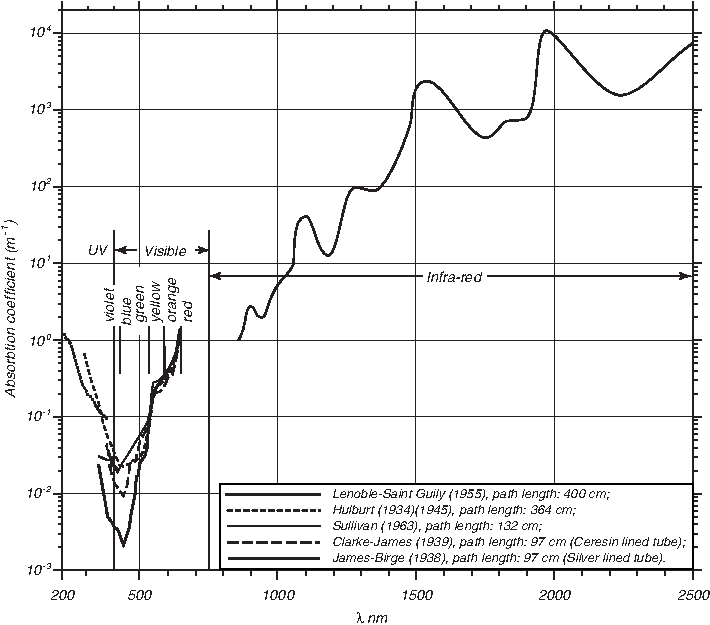
\includegraphics{attenuation}}
%% \footnotesize
%% Figure 6.17 Absorption \rule{0mm}{3ex}coefficient for pure water as a
%% function of wavelength $\lambda$ of the radiation. Redrawn from Morel
%% (1974: 18, 19). See Morel (1974) for references.
%% 
%% \label{fig:attenuation}
%% \vspace{-4ex}
%% \end{figure}

Скорость затухания солнечного света в воде определяет глубину, до которой
океан освещается и нагревается Солнцем. Причиной этого затухания служит
абсорбция света пигментами, а также его рассеивание молекулами самой воды 
%% Доронин указывает и другие поглотители, кроме пигментов: ионы солей,
%% желтое вещество
и взвешенными в ней частицами. Характер затухания определяется длиной волны
излучения: так, голубая часть спектра наименее подвержена поглощению, а
красная, наоборот, поглощается сильнее всего. Затухание на единицу расстояния
пропорционально энергетической яркости и энергетической освещенности света:
\begin{equation}
\frac{dI}{dx} = -c \, I,
\end{equation}
где $x$~--- расстояние вдоль луча, $c$~--- коэффициент затухания 
(рис.~6.17), а $I$~--- яркость или освещённость.
%
% The rate at which sunlight is attenuated determines the depth which is
% lighted and heated by the sun. Attenuation is due to absorption by
% pigments and scattering by molecules and particles. Attenuation
% depends on wavelength.  Blue light is absorbed least, red light is
% absorbed most strongly.  Attenuation per unit distance is proportional
% to the radiance or the irradiance of light:
% \begin{equation}
% \frac{dI}{dx} = -c \, I
% \end{equation}
% where $x$ is the distance along beam, $c$ is an attenuation
% coefficient (figure 6.17), and $I$ is irradiance or radiance.

\emph{Энергетическая яркость}~--- отношение потока излучения, 
распространяющегося в малом телесном углу и принимаемого малым элементом 
поверхности, к произведению площади элемента и величины угла соответственно.%
\remark{\url{http://slovari.yandex.ru/dict/bse/article/00095/09600.htm}}
Эта характеристика используется для описания энергии в потоке света, 
приходящем с определённого направления. Иногда мы хотим знать, сколько света
достигает некоторой глубины в океане, не принимая во внимание
направление, с которого он приходит. В этом случае мы используем
\emph{энергетическую освещённость} в точке поверхности~--- <<отношение 
потока излучения, падающего на малый элемент поверхности, 
содержащий рассматриваемую точку, к площади этого элемента>>%
\remark{\url{http://slovari.yandex.ru/dict/bse/article/00055/92300.htm}}. 
%
% \textit{Radiance} \index{radiance|textbf}is the power per unit area
% per solid angle. It is useful for describing the energy in a beam of
% light coming from a particular direction.  Sometimes we want to know
% how much light reaches some depth in the ocean regardless of which
% direction it is going. In this case we use
% \textit{irradiance}\index{irradiance|textbf}, which is the power per
% unit area of surface.

Если коэффициент поглощения постоянен, энергетическая яркость
экспоненциально уменьшается с расстоянием:
\begin{equation}
I_2 = I_1 \: \exp(-cx),
\end{equation}
где $I_1$~--- первоначальная энергетическая яркость либо освещённость,
а $I_2$~--- значение этой же характеристики после поглощения.
%
% If the absorption coefficient is constant, the light intensity
% decreases exponentially with distance.
% \begin{equation}
% I_2 = I_1 \: \exp(-cx)
% \end{equation}
% where $I_1$ is the original radiance or irradiance of light, and $I_2$
% is the radiance or irradiance of light after absorption.

\begin{paragraph}{Прозрачность воды в океане.} 
Морская вода в центре океана очень прозрачна, даже прозрачнее, чем 
дистиллированная. Цвет этой воды~--- темно-голубой, кобальтовый, почти чёрный.
Благодаря этому, течение, текущее на север вдоль побережья Японии, которое 
несет очень прозрачные воды из центра Тихого океана в высокие широты, 
получило своё название Куросио (яп. <<чёрное течение>>).
Наиболее прозрачная океанская вода называется водой типа~I по классификации 
Ерлова (рис. 6.18). Эта вода настолько чиста, что 10\% света, проходящего 
через поверхность, достигает глубины~$90\m$.
%
% \textit{Clarity of Ocean Water} \index{water!clarity of|textbf}Sea
% water in the middle of the ocean is very clear---clearer than
% distilled water. These waters are a very deep, cobalt, blue---almost
% black. Thus the strong current which flows northward offshore of Japan
% carrying very clear water from the central Pacific into higher
% latitudes is known as the Black Current, or Kuroshio\index{Kuroshio}
% in Japanese. The clearest ocean water is called Type I waters by
% Jerlov (figure 6.18). The water is so clear that 10\% of the light
% transmitted below the sea surface reaches a depth of 90 m.

%% \begin{figure}[t!]
%% \makebox [120mm][c]{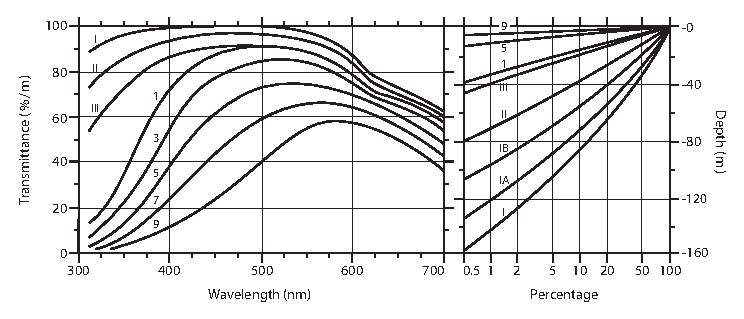
\includegraphics{jerlov}}
%% \footnotesize
%% Figure 6.18 \textbf{Left:} Transmittance \rule{0mm}{3ex}of daylight in
%% the ocean in \% per meter as a function of wavelength. I: extremely
%% pure ocean water; II: turbid tropical-subtropical water; III:
%% mid-latitude water; 1-9: coastal waters of increasing
%% turbidity. Incidence angle is 90\degrees for the first three cases,
%% 45\degrees for the other cases. \textbf{Right:} Percentage of 465 nm
%% light reaching indicated depths for the same types of water. After
%% Jerlov (1976).
%% \label{fig:jerlov}
%% \vspace{-3ex}
%% \end{figure}

В субтропиках и средних широтах морская вода, близкая к побережью,
содержит больше фитопланктона, чем очень прозрачные воды в центре
океана. Хлорофилл в фитопланктоне поглощает свет, а сами растения его
рассеивают. Вместе эти процессы изменяют наблюдаемый цвет
океана. Очень продуктивные воды с большой концентрацией
фитопланктона имеют голубовато-зелёный или зелёный цвет (рис.~6.19).
В безоблачную погоду цвет океана можно наблюдать из
космоса. Это позволяет сканерам цвета океана, таким как SeaWiFS,
картировать распределение фитопланктона на больших пространствах.
%
% In the subtropics and mid-latitudes closer to the coast, sea water
% contains more phytoplankton than the very clear central-ocean
% waters. Chlorophyll pigments in phytoplankton absorb light, and the
% plants themselves scatter light. Together, the processes change the
% color of the ocean as seen by observer looking downward into the
% sea. Very productive waters, those with high concentrations of
% phytoplankton, appear blue-green or green (figure 6.19). On clear days
% the color can be observed from space. This allows ocean-color
% scanners, such as those on SeaWiFS, to map the distribution of
% phytoplankton over large areas.

При увеличении концентрации фитопланктона, глубина, на которой
солнечный свет полностью поглощается, уменьшается. Более мутные
тропические и среднеширотные воды относятся по классификации Ерлова
к типам~II и~III (рис.~6.18). Таким образом, глубина, до которой
солнечный свет нагревает воду, зависит от её продуктивности. Это
усложняет расчёт солнечного прогрева перемешанного слоя.
%
% As the concentration of phytoplankton increases, the depth where
% sunlight is absorbed in the ocean decreases. The more turbid tropical
% and mid-latitude waters are classified as type II and III waters by
% Jerlov (figure 6.18). Thus the depth where sunlight warms the water
% depends on the productivity of the waters. This complicates the
% calculation of solar heating of the mixed layer\index{mixed
% layer!solar heating and phytoplankton}.

Чем ближе вода к берегу, тем менее она прозрачна. Воды, находящиеся у
самого побережья, относятся к показанным на рис.~6.18 типам 1--9.
Они содержат пигменты, принесенные с суши, иногда называемые
гельбштоф, что просто означает <<жёлтое вещество>>, мутную речную воду и
ил, поднятый волнами на мелководье. Лишь небольшое количество света 
проходит в этих водах глубже нескольких метров.
%
% Coastal waters are much less clear than waters offshore. These are the
% type 1--9 waters shown in figure 6.18. They contain pigments from
% land, sometimes called gelbstoffe, which just means yellow stuff,
% muddy water from rivers, and mud stirred up by waves in shallow
% water. Very little light penetrates more than a few meters into these
% waters.

%% \begin{figure}[t!]
%% \makebox [120mm][c]{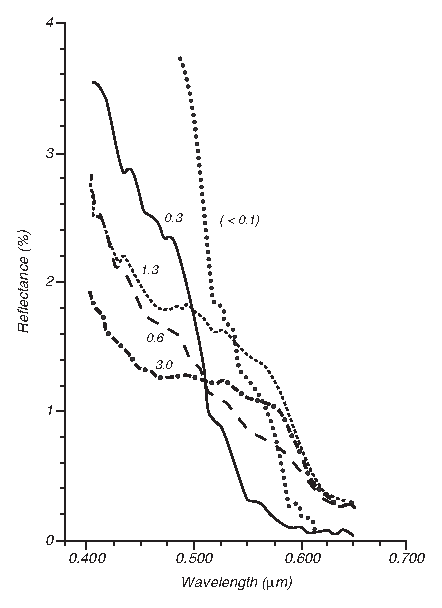
\includegraphics{reflectance}}
%% \footnotesize
%% Figure 6.19 Spectral \rule{0mm}{4ex}reflectance of sea water observed
%% from an aircraft flying at 305 m over waters of different colors in
%% the Northwest Atlantic. The numerical values are the average
%% chlorophyll concentration in the euphotic (sunlit) zone in units of
%% mg/m$^3$. The reflectance is for vertically polarized light observed
%% at Brewster's angle of 53\degrees. This angle minimizes reflected
%% skylight and emphasizes the light from below the sea surface. After
%% Clarke, Ewing, and Lorenzen (1970).
%% \label{fig:reflectance}
%% \vspace{-3ex}
%% \end{figure}

%% Рисунок 6.19 Коэффициент ослабления c и коэффициент рассеивания b для
%% чистой воды как функция длинны волны l излучения (Взято из Dietrich,
%% et al. 1980).
%%
%% Рисунок 6.20 Слева: ослабление дневного света в океане в \% на метр
%% как функция длины волны I: очень чистый океан; II: мутные тропические
%% и субтропические воды; III: среднеширотные воды; 1--9: прибрежные воды
%% увеличивающейся замутнённости. Угол падения для первых трёх случаев
%% $\degrees{90}$ для остальных случаев $\degrees{45}$. (Взято из Jerlov,
%% 1951). Справа: Количество света с длиной волны 465~нм достигающего
%% определённой индикаторной глубины в тех же типах воды. (Взято из
%% Jerlov, 1968).
%% 
%% Рисунок 6.21 Спектральная отражательная способность морской воды
%% полученная в результате пролёта самолёта на высоте 305 м над водами с
%% разной цветностью в Северозападной Атлантике. Численные значения~---
%% среднее содержание хлорофила в фотической зоне в мг/м3. Отражательная
%% способность дана для вертикально поляризованного света наблюдаемого
%% под углом Брюстера~--- $\degrees{53}$. Этот угол минимизирует отражённый от
%% поверхности свет и выделяет свет из подповерхностных слоёв. (Взято из
%% Clarke, Ewing, и Lorenzen, 1970).
\end{paragraph}

\begin{paragraph}{Измерение хлорофилла из космоса.}
% \paragraph{Measurement of Chlorophyll from Space}
Цвет океана, а следовательно, и концентрация хлорофилла в его верхних слоях,
была измерена с помощью инструмента Coastal Zone Color Scanner, установленного
на спутнике Nimbus-7, который был запущен в~1978~г., Sea-viewing Wide
Field-of-view Sensor (SeaWiFS), установленного на спутнике SeaStar,
запущенном в 1997~г., и Moderate Resolution Imaging Spectrometer (MODIS),
установленного на спутниках Terra и~Aqua, запущенных в 1999 и~2002~гг.\ %
соответственно. MODIS измеряет upwelling radiance в 36 диапазонах длин
волн от~$405\nm$ до~$14\,385\nm$.
%% upwelling radiance --- "восходящее излучение"???
%
% \index{chlorophyll!measurement from space}The color of the ocean, and
% hence the chlorophyll concentration in the upper layers of the ocean
% has been measured by the Coastal Zone Color Scanner carried on the
% Nimbus-7 satellite launched in 1978, by the Sea-viewing Wide
% Field-of-view Sensor (SeaWiFS) carried on SeaStar, launched in 1997,
% and on the Moderate Resolution Imaging Spectrometer
% (\textsc{modis})\index{MODIS} carried on the Terra\index{Terra
% satellite} and Aqua\index{Agua satellite} satellites launched in 1999
% and 2002 respectively. \textsc{modis} measures
% upwelling\index{upwelling!radiance} radiance in 36 wavelength bands
% between 405 nm and 14,385 nm.

Большая часть наблюдаемого со спутника upwelling radiance приходит из
атмосферы, а лишь около 10\%~--- от поверхности моря. И молекулы
воздуха, и аэрозоли рассеивают свет; для устранения влияния атмосферы
были разработаны очень точные методы. 
%% вариант: "требующие высокой точности (тщательности) методы"?
%
% Most of the upwelling radiance seen by the satellite comes from the
% atmosphere. Only about 10\% comes from the sea surface. Both air
% molecules and aerosols scatter light, and very accurate techniques
% have been developed to remove the influence of the atmosphere.

Полное излучение~$L_t$, принимаемое прибором, представляет собой
\begin{equation}
 L_t(\lambda_i) = t(\lambda_i)L_W(\lambda_i) + L_r(\lambda_i) + L_a(\lambda_i),
\end{equation}
где $\lambda_i$~--- длина волны излучения в диапазоне, который измеряется
данным инструментом, $L_W$~--- излучение, исходящее с поверхности моря, 
$L_r$~--- рассеянное молекулами (называемое также рэлеевской радиацией), 
$L_a$~--- рассеянное аэрозолями, а $t$~--- коэффициент прозрачности атмосферы. 
Величина~$L_r$ может быть рассчитана теоретически, а $L_a$~--- исходя
из количества принятого инструментом красного света, поскольку лишь
малое его количество отражается от поверхности воды. Следовательно,
значение~$L_W$ может быть определено по излучению, измеряемому спутником. 
%
% The total radiance $L_t$ received by an instrument in space is:
% \begin{equation}
% L_t(\lambda_i) = t(\lambda_i)L_W(\lambda_i)+L_r(\lambda_i)+L_a(\lambda_i)
% \end{equation}
% where $\lambda_i$ is the wavelength of the radiation in the band
% measured by the instrument, $L_W$ is the radiance leaving the sea
% surface, $L_r$ is radiance scattered by molecules, called the Rayleigh
% radiance, $L_a$ is radiance scattered from aerosols, and $t$ is the
% transmittance of the atmosphere. $L_r$ can be calculated from theory,
% and $L_a$ can be calculated from the amount of red light received at
% the instrument because very little red light is reflected from the
% water. Therefore $L_W$ can be calculated from the radiance measured at
% the spacecraft.

Концентрация хлорофилла в столбе воды рассчитывается, исходя
из отношения величин~$L_W$ в двух частотных диапазонах. Используя данные с
Coastal Zone Color Scanner, Gordon et al. (1983) предложили:
\begin{subequations}
\begin{align}
C_{13} &= 1.1298 \left[\frac{L_W(443)}{L_W(550)}\right]^{-1.71}\\
C_{23} &= 3.3266 \left[\frac{L_W(520)}{L_W(550)}\right]^{-2.40}
\end{align}
\end{subequations}
где $C$~--- концентрация хлорофилла в поверхностных слоях, выраженная в~$\mg$
пигмента на $1\cubm$, а $L_W(443)$, $L_W(520)$, и~$L_W(550)$~--- излучение на
длинах волн $443$, $520$, и~$550\nm$. Величина~$C_{13}$ используется,
когда~$C_{13}\le 1.5\mgpcm$; в других случаях используют~$C_{23}$.  
Этот способ позволяет рассчитывать концентрацию хлорофилла с точностью~50\% 
в широком диапазоне от~$0.01$ до~$10\mgpcm$.
%
% Chlorophyll concentration \index{chlorophyll!calculating
% concentration}in the water column is calculated from the ratio of
% $L_W$ at two frequencies. Using data from the Coastal Zone Color
% Scanner, Gordon et al. (1983) proposed
% \begin{subequations}
% \begin{align}
% C_{13} = & 1.1298 \left[ \frac{L_W(443)}{L_W(550)}\right]^{-1.71}\\
% C_{23} = & 3.3266 \left[ \frac{L_W(520)}{L_W(550)}\right]^{-2.40}
% \end{align}
% \end{subequations}
% where $C$ is the chlorophyll concentration in the surface layers in mg
% pigment/m$^3$, and $L_W(443), L_W(520), and L_W(550)$ is the radiance
% at wavelengths of 443, 520, and 550 nm.  $C_{13}$ is used when 
% $C_{13} \le 1.5$ mg/m$^3$, otherwise $C_{23}$ is used.
%
% The technique is used to calculate chlorophyll concentration within a
% factor of 50\% over a wide range of concentrations from 0.01 
% to 10 mg/m$^3$.
\end{paragraph}
\end{section}

\begin{section}{Основные концепции}
% \section{Important Concepts}
\begin{enumerate}
\item
Плотность воды в океане определяется температурой, солёностью и давлением.
%
% Density in the ocean is determined by temperature, salinity, and
% pressure.
   
\item
Изменения плотности в океане очень малы; изучение водных масс и
течений требует точности измерений до 10 частей на миллион.
%
% Density changes in the ocean are very small, and studies of water
% masses and currents require density with an
% accuracy\index{accuracy!density} of 10 parts per million.

\item
Плотность не измеряется, а рассчитывается по данным о температуре, 
солёности и давлении с помощью уравнения состояния морской воды.
%
% Density is not measured, it is calculated from measurements of
% temperature, salinity, and pressure using the equation of state of sea
% water.


\item
Для точного вычисления плотности необходимы точные определения
температуры и солёности, а также точное уравение состояния.
%
% Accurate calculations of density require accurate definitions of
% temperature and salinity and an accurate equation of state.

\item
Существуют определенные сложности как с формулировкой определения понятия
солёности, так и с её измерением. Чтобы устранить эти затруднения, вместо 
солёности океанографы используют электропроводность. Плотность воды, таким
образом, вычисляется по её электропроводности, температуре и давлению.
%
% Salinity is difficult to define and to measure. To avoid the
% difficulty, oceanographers use conductivity instead of salinity. They
% measure conductivity and calculate density from temperature,
% conductivity, and pressure.

\item
Перемешанный слой с постоянной температурой и солёностью обычно
находится в верхних слоях океана глубиной~$1$--$100\m$. Конкретная толщина 
перемешанного слоя определяется скоростью ветра и потоком тепла через 
поверхность.
%
% A mixed layer\index{mixed layer} of constant temperature and salinity
% is usually found in the top 1--100 meters of the ocean. The depth is
% determined by wind speed and the flux of heat through the sea surface.

\item
Чтобы сравнивать температуру и плотность водных масс на разных
глубинах, океанографы используют потенциальную температуру и
потенциальную плотность, которые почти полностью устраняют влияние давления
на плотность.
%
% To compare temperature and density of water masses at different depths
% in the ocean, oceanographers use potential temperature and potential
% density which remove most of the influence of pressure on density.

\item 
Частицы воды на глубинах, превышающих толщину перемешанного слоя, перемещаются
вдоль нейтральных поверхностей.
%
% Water parcels below the mixed layer\index{mixed layer} move along
% neutral surfaces.

\item
Температура поверхности океана обычно измерялась с использованием
bucket (ведёрной) или инжекторной температуры. На глобальных картах
температуры эти наблюдения объединяются с данными об инфракрасном
излучении морской поверхности, полученными при помощи спутникового 
инструмента~AVHRR.
%
% Surface temperature of the ocean was usually measured at sea using
% bucket or injection temperatures. Global maps of temperature combine
% these observations with observations of infrared radiance from the sea
% surface measured by an \textsc{avhrr} \index{Advanced Very High
% Resolution Radiometer (AVHRR)}in space.

\item
Температура и солёность как функция давления обычно измеряются электронным 
способом с помощью CTD. До 1960--1970~гг.\ солёность и температуру 
измеряли примерно на 20 уровнях глубины при помощи батометров
Нансена, погружаемых с корабля на тросе. Эти батометры несли на себе
опрокидывающиеся термометры, которые регистрировали температуру и глубину 
погружения, а также доставляли на поверхность пробу воды, которая затем
использовалась на борту корабля для определения солёности.
%
% Temperature and conductivity are usually measured digitally as a
% function of pressure using a \textsc{ctd}\index{CTD}. Before
% 1960--1970 the salinity and temperature were measured at roughly 20
% depths using Nansen bottles lowered on a line from a ship. The bottles
% carried reversing thermometers\index{thermometer!reversing} which
% recorded temperature and depth and they returned a water sample from
% that depth which was used to determine salinity on board the ship.

\item
Свет быстро поглощается океаном. Даже в самой прозрачной морской воде 
около~95\% солнечного света абсорбируется на глубине до~$100\m$, 
а в мутных прибрежных водах солнечный свет редко проникает глубже нескольких
метров.
%
% Light is rapidly absorbed in the ocean. 95\% of sunlight is absorbed
% in the upper 100 m of the clearest sea water. Sunlight rarely
% penetrates deeper than a few meters in turbid coastal waters.

\item
Фитопланктон изменяет цвет морской воды; эти изменения можно
проследить из космоса и определить по ним концентрацию фитопланктона. 
%
% Phytoplankton change the color of sea water, and the change in color
% can be observed from space. Water color is used to measure
% phytoplankton concentration from space.
\end{enumerate}
\end{section}
\end{chapter}
